\chapter{Wyniki badań i~ich analiza}
\label{c:badania}

Wyniki, jakie otrzymano z~przeprowadzonych eksperymentów pozwalają określić, czy badany problem rozpoznawania brył może zostać rozwiązany z~użyciem metod uczenia głębokiego. Niniejszy rozdział prezentuje uzyskane wyniki oraz ich analizę. Przeprowadzono w~nim również analizę najczęstszych błędów modeli i~wysnuto wnioski dlaczego~\nobreakdash{zachodzą}.

Do przeprowadzenia eksperymentów wytrenowano siedem sieci o~architekturze YOLO, wykorzystując ten sam zbiór danych, korzystając z~procesorów graficznych firmy NVIDIA. W~części eksperymentów obrazy przed treningiem przekształcono do odcieni szarości zgodnie z~procedurą opisaną w~\ref{ssec:filtry}. Macierz wariantów modeli została przedstawiona w~tabeli~\ref{tab:exp_matrix}. Taka liczba modeli pozwala na przeprowadzenie eksperymentów założonych w~sekcji \ref{ssec:procedure}.

\begin{table}[ht]
    \centering
    \caption{Macierz modeli wytrenowanych w~ramach badań.}
    \label{tab:exp_matrix}
    \begin{tabular}{l|cccc}
        \toprule
        \textbf{Model} & \textbf{RGB 640} & \textbf{RGB 1024} & \textbf{grayscale 640} & \textbf{grayscale 1024} \\
        \midrule
        YOLO26n        & \checkmark       & \checkmark        & \checkmark             & \checkmark              \\
        YOLO26s        & \checkmark       & \checkmark        & \checkmark             &                         \\
        \bottomrule
    \end{tabular}
\end{table}

\section{Zestawienie wyników treningów} % 6.1

Każdy z~wytrenowanych modeli został oceniony pod kątem jakości detekcji na zbiorze testowym. Do oceny jakości detekcji za każdym razem wykorzystano model, który w~trakcie uczenia osiągnął najlepsze wyniki na zbiorze walidacyjnym. Kryterium wyboru najlepszego modelu była wartość $mAP50\text{-}95$. Po przeprowadzeniu treningu każdy z~modeli został oceniony na zbiorze testowym, a~wyniki zostały zestawione w~tabeli~\ref{tab:results}.

\begin{table}[ht]
    \centering
    \footnotesize
    \caption{Zestawienie wyników detekcji modeli na zbiorze testowym.}
    \label{tab:results}
    \begin{tabular}{l|ccccccc}
        \toprule
        \textbf{ID}              & $E_1$    & $E_2$    & $E_3$   & $E_4$   & $E_5$     & $E_6$     & $E_7$     \\
        \midrule
        \textbf{Model}           & YOLO26n  & YOLO26s  & YOLO26n & YOLO26s & YOLO26n   & YOLO26s   & YOLO26n   \\
        \textbf{Dane}            & RGB      & RGB      & RGB     & RGB     & grayscale & grayscale & grayscale \\
        \textbf{Rozmiar obrazu}  & 640      & 640      & 1024    & 1024    & 640       & 640       & 1024      \\
        \textbf{Ostatnia epoka}  & 190      & 108      & 211     & 114     & 203       & 280       & 230       \\
        \textbf{Najlepsza epoka} & 140      & 60       & 161     & 64      & 153       & 230       & 180       \\
        \midrule
        \textbf{Precision}       & 0.714    & 0.701    & 0.794   & 0.846   & 0.591     & 0.630     & 0.649     \\
        \textbf{Recall}          & 0.678    & 0.760    & 0.825   & 0.736   & 0.475     & 0.601     & 0.601     \\
        $mAP50$                  & 0.716    & 0.786    & 0.862   & 0.844   & 0.488     & 0.560     & 0.621     \\
        $mAP50\text{-}95$        & 0.599    & 0.641    & 0.719   & 0.729   & 0.360     & 0.449     & 0.495     \\
        \textbf{$F1$-score}      & 0.696    & 0.730    & 0.809   & 0.787   & 0.526     & 0.615     & 0.624     \\
        \midrule
        \textbf{GPU}             & RTX 4060 & RTX 4060 & L40S    & L40S    & A100      & A100      & A100      \\
        \bottomrule
    \end{tabular}
\end{table}

Prawie każdy z~treningów zakończył się jego wcześniejszym zatrzymaniem, co oznacza, że w~trakcie uczenia model osiągnął wartość $mAP50\text{-}95$ na zbiorze walidacyjnym, która nie uległa poprawie przez 50 kolejnych epok. Uczenie modelu $E_2$ zakończono po 48 epokach bez poprawy wartości ze względu na ograniczenia czasowe dostępu do jednostki obliczeniowej i~nie podjęto decyzji o~kontynuacji treningu. Trening wariantu \texttt{s} na obrazach kolorowych w~obu przypadkach ($E_2$, $E_4$) potrzebował mniejszej liczby epok do osiągnięcia najlepszej wartości kryterium walidacyjnego niż wariant \texttt{n} ($E_1$, $E_3$).

Większość treningów modeli miała stabilny przebieg, charakteryzujący się szybkim wzrostem wartości metryk mAP, a~następnie ich wypłaszczenie. Jest to typowe zachowanie w~procesie uczenia modeli YOLO, które w~początkowej fazie szybko dopasowują się do danych treningowych, a~następnie optymalizują wagi w~celu poprawy jakości detekcji. Przebieg treningu modelu $E_1$ wraz ze zmianami wartości jego metryk został przedstawiony na rysunku~\ref{fig:training_curve}. Możemy na nim zaobserwować, że wartości funkcji straty dla zbioru uczącego systematycznie maleją, co świadczy o~tym, że model uczy się coraz lepiej dopasowywać do danych treningowych. Podobne tendencje, choć nie tak wyraźne, obserwujemy w~przypadku wartości funkcji straty dla zbioru walidacyjnego. Jednocześnie wartości metryk jakości detekcji szybko rosną świadcząc o~tym, że model coraz lepiej dopasowuje etykiety do obiektów na obrazach.

\begin{figure}[htbp]
    \centering
    \begin{subfigure}{\textwidth}
        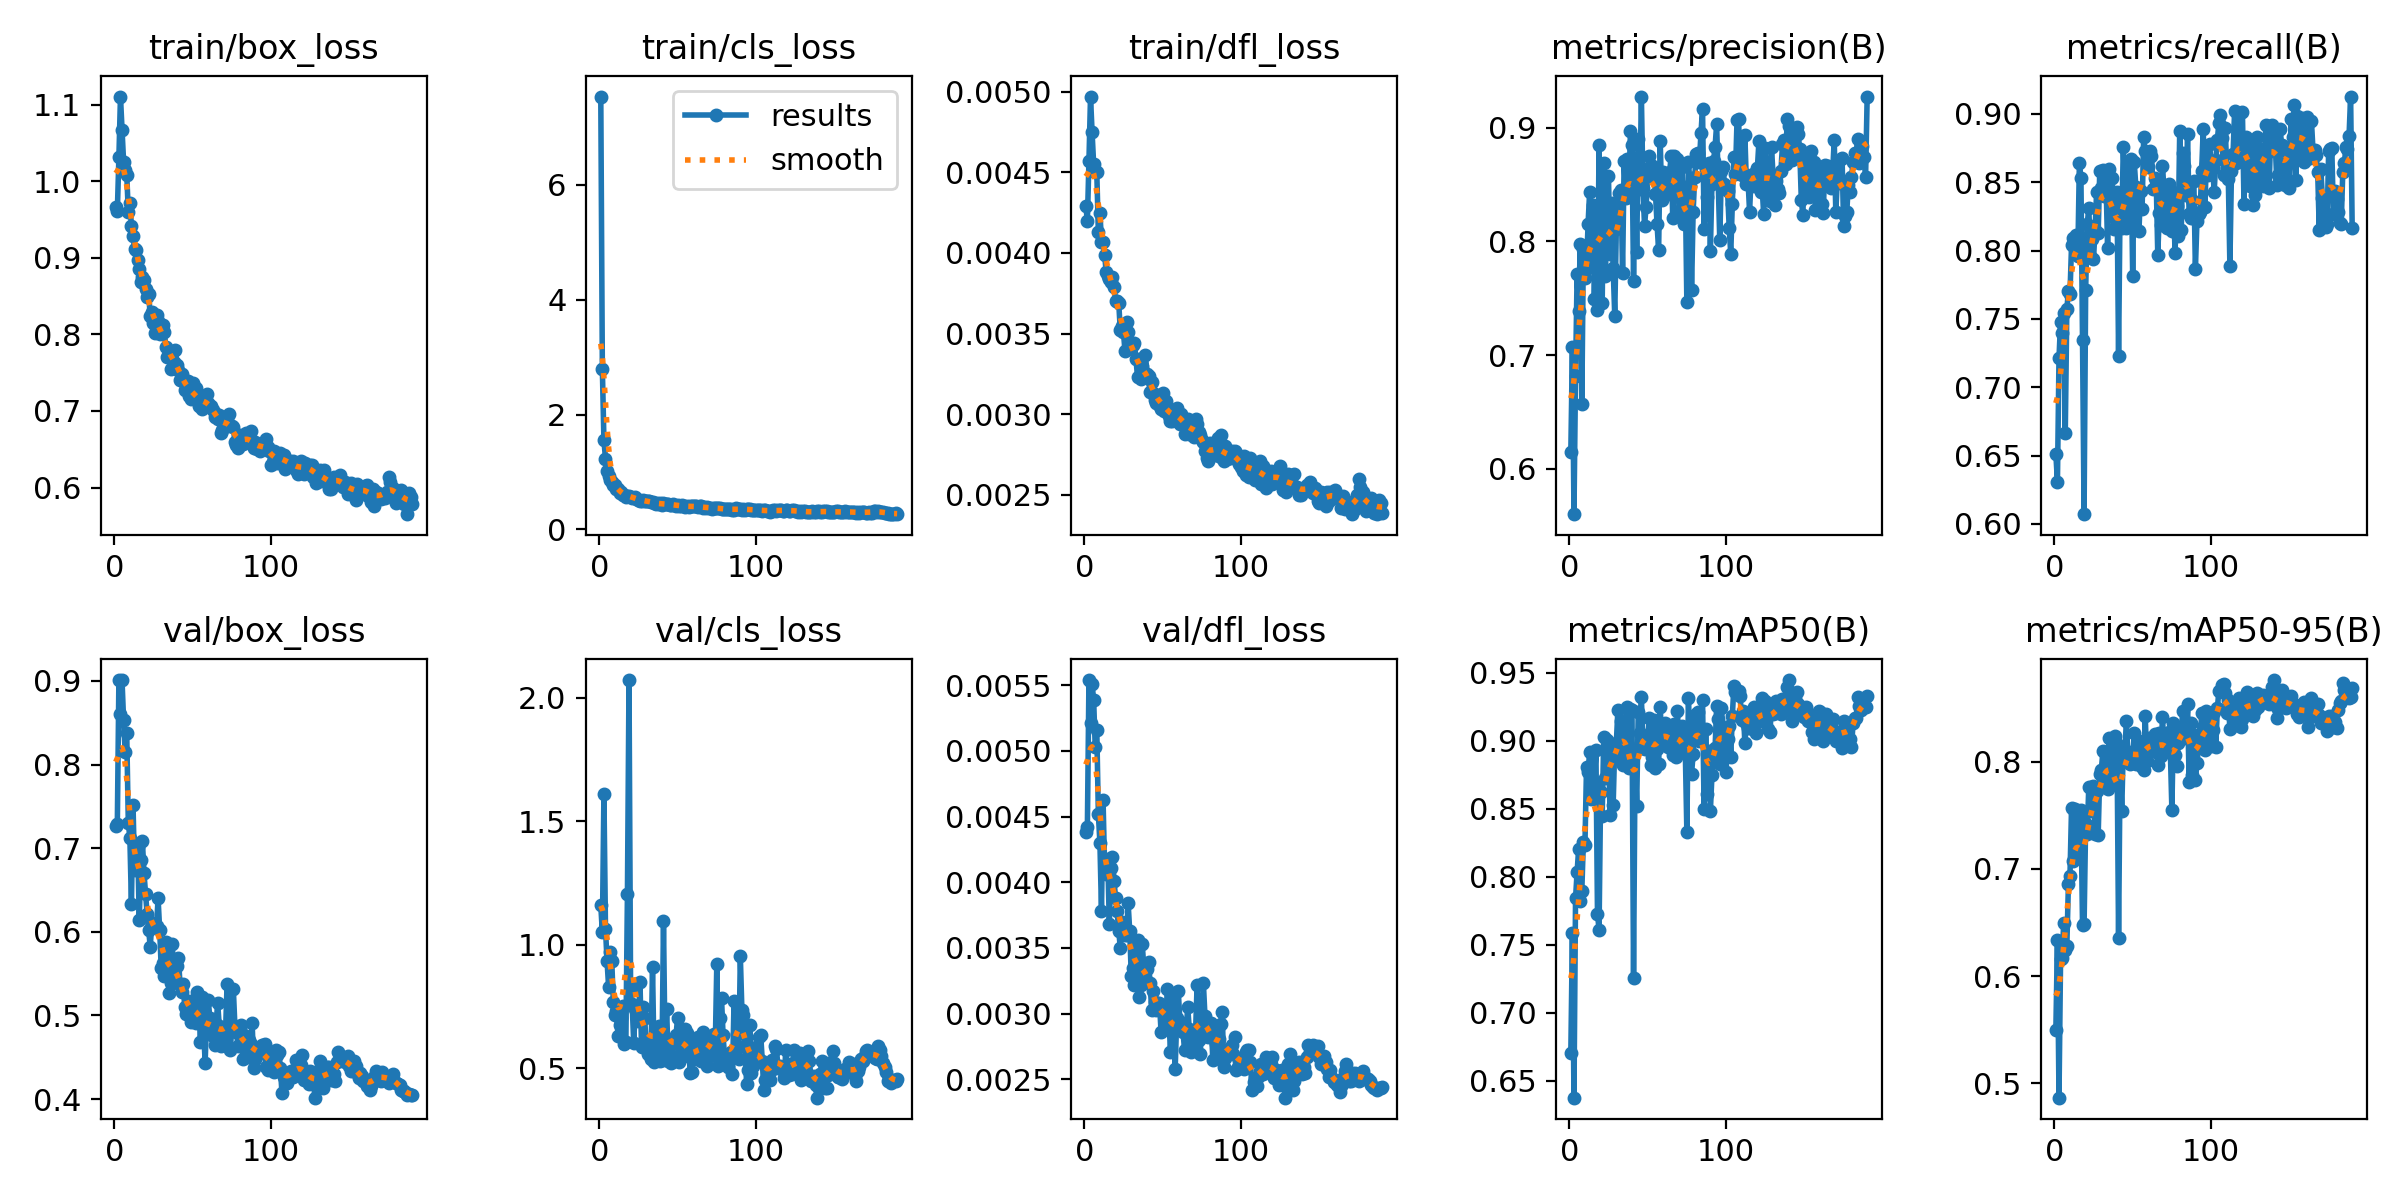
\includegraphics[width=\textwidth]{./graf/yolo26n_640_rgb_results.png}
        \caption{Przebieg treningu wariantu $E_1$.}
        \label{fig:training_curve}
    \end{subfigure}

    \vspace{1cm}

    \begin{subfigure}{\textwidth}
        \includegraphics[width=\textwidth]{./graf/yolo26s_640_rgb_results.png}
        \caption{Przebieg treningu wariantu $E_2$.}
        \label{fig:training_curve_e2}
    \end{subfigure}
    \caption{Przebiegi treningu modeli YOLO26 na obrazach kolorowych o~rozdzielczości 640 pikseli.}
\end{figure}

Ciekawym przypadkiem jest trening modelu $E_2$, który osiągnął najlepszą wartość metryki w~60. epoce. Analiza przebiegu uczenia, ukazanego na rysunku~\ref{fig:training_curve_e2}, pokazuje, że w~trakcie treningu wystąpiło nagłe załamanie wartości metryk jakości detekcji. Pomimo systematycznego spadku wartości funkcji straty, od około połowy treningu funkcja straty na zbiorze walidacyjnym zaczęła wzrastać. W~końcowej fazie treningu widzimy jednak powrót do klasycznego przebiegu uczenia, co może skłaniać do przeprowadzenia dalszych badań nad tym przypadkiem. Obserwowany przebieg uzasadniałby ponowienie treningu modelu $E_2$ w~celu sprawdzenia, czy wzrost metryk walidacyjnych utrzymałby się w~kolejnych epokach.

\section{Wpływ skali modelu na jakość detekcji} % 6.2

Aby ocenić wpływ skali modelu na jakość detekcji, w~eksperymencie A~porównano modele YOLO26n i~YOLO26s. W~tym celu wykorzystano modele wytrenowane na obrazach kolorowych o~rozdzielczościach 640 ($E_1$, $E_2$) oraz 1024 pikseli ($E_3$, $E_4$). Wyniki zestawiono parami, tak aby w~każdym porównaniu jedyną zmienną była skala modelu. Wartości metryk dla poszczególnych porównań przedstawiono w~tabeli~\ref{tab:exp_a}.

\begin{table}[ht]
    \centering
    \caption{Porównanie jakości wariantów modeli YOLO26 n i~s w~eksperymencie A.}
    \label{tab:exp_a}
    \begin{tabular}{l|ccc|ccc}
        \toprule
        \multirow{2}{*}{\textbf{Metryka}}
         & \multicolumn{3}{c|}{\textbf{RGB 640}}
         & \multicolumn{3}{c}{\textbf{RGB 1024}}                           \\
        \cline{2-7}
         & YOLO26n                               & YOLO26s & Różnica (s-n)
         & YOLO26n                               & YOLO26s & Różnica (s-n) \\
        \midrule
        $mAP50$
         & 0.71595                               & 0.78551 & +0.06957
         & 0.86231                               & 0.84409 & -0.01823      \\

        $mAP50\text{-}95$
         & 0.59866                               & 0.64119 & +0.04253
         & 0.71856                               & 0.72932 & +0.01077      \\

        $F1$-score
         & 0.69568                               & 0.73041 & +0.03473
         & 0.80908                               & 0.78712 & -0.02195      \\
        \bottomrule
    \end{tabular}
\end{table}

Dla obrazów o~rozdzielczości 640 pikseli wyższą wartość analizowanych metryk osiągnął wariant \texttt{s}. Wartość $mAP50$ uległa poprawie o~$6,96$ p.p. (punktu procentowego), a~dla bardziej rygorystycznej $mAP50\text{-}95$ różnica wyniosła około $4,25$ p.p. Wartość wskaźnika $F1$-score również wzrosła, co wskazuje, że w~takiej konfiguracji większy model wykazuje się lepszą jakością detekcji na zbiorze testowym.

Inną zależność obserwujemy przy większych obrazach wejściowych o~rozdzielczości 1024 pikseli. Model YOLO26s uzyskał nieznacznie wyższą wartość $mAP50\text{-}95$, o~$1,08$ p.p. Jednocześnie, mniejszy wariant osiągnął wyższe wartości $mAP50$ i~wskaźnika $F1$-score. Oznacza to, że przy większym obrazie wejściowym wzrost skali modelu nie przekłada się bezpośrednio na poprawę jakości detekcji.

Porównanie obu rozdzielczości wskazuje, że wpływ zwiększenia skali modelu zależy od rozmiaru obrazu wejściowego. Dla mniejszych obrazów lepszą jakość detekcji wykazuje model YOLO26s. Przy obrazach o~rozdzielczości 1024 pikseli korzyść użycia większego modelu widoczna jest jedynie w~wartości metryki $mAP50\text{-}95$. Można więc zauważyć, że zwiększenie skali modelu ma większe znaczenie przy korzystaniu z~mniejszych obrazów wejściowych, natomiast przy większej ilości danych na wejściu przewaga większego wariantu ulega znacznemu ograniczeniu.

Wyniki eksperymentu A~nie wskazują więc na stałą przewagę jednego wariantu, a~raczej na zależność jakości detekcji od ilości informacji dostarczanych modelowi. YOLO26s przynosi znaczną poprawę dla mniejszych obrazów, lecz dla wariantu 1024 oba modele zachowują podobne właściwości detekcji. Ocena zasadności użycia większego wariantu modelu wymaga więc uwzględnienia również innych czynników, takich jak koszt obliczeniowy i~czas inferencji, które zostaną zestawione w~kolejnych sekcjach rozdziału.

\section{Wpływ rozdzielczości obrazu wejściowego na jakość detekcji} % 6.3

W~kolejnym eksperymencie badano wpływ rozmiaru wejściowego obrazu na jakość detekcji, porównując ze sobą modele trenowane na obrazach kolorowych z~parametrem \texttt{imgsz} ustawionym na 640 i~1024 piksele. Do porównania wykorzystano pary modeli o~tej samej skali, tak aby możliwe było wyizolowanie wpływu rozdzielczości obrazu wejściowego na jakość detekcji. Wyniki porównania zestawiono w~tabeli~\ref{tab:exp_b}.

Przykład wpływu rozdzielczości obrazu wejściowego przedstawiono na rysunku~\ref{fig:img_resize}. W~prezentowanym przypadku w~wariancie 640 bryła jest reprezentowana przez $11730$ pikseli, a~w~wariancie 1024 przez $29646$ pikseli. Stanowi to wzrost o~$2,53$ razy i~może wpływać na zdolność modelu do wykrywania obiektów, szczególnie w~przypadku mniejszych brył. Warto jednak zauważyć, że zwiększenie rozdzielczości obrazu wejściowego niesie za sobą również zwiększony koszt obliczeniowy oraz wydłużenie czasu inferencji.

\begin{table}[ht]
    \centering
    \caption{Porównanie jakości modeli dla rozmiarów obrazu wejściowego 640 i~1024 pikseli w~eksperymencie B.}
    \label{tab:exp_b}
    \begin{tabular}{l|ccc|ccc}
        \toprule
        \multirow{2}{*}{\textbf{Metryka}}
         & \multicolumn{3}{c|}{\textbf{YOLO26n}}
         & \multicolumn{3}{c}{\textbf{YOLO26s}}                       \\
        \cline{2-7}
         & 640                                   & 1024    & Różnica
         & 640                                   & 1024    & Różnica  \\
        \midrule
        $mAP50$
         & 0.71595                               & 0.86231 & +0.14636
         & 0.78551                               & 0.84409 & +0.05857 \\

        $mAP50\text{-}95$
         & 0.59866                               & 0.71856 & +0.11990
         & 0.64119                               & 0.72932 & +0.08813 \\

        $F1$-score
         & 0.69568                               & 0.80908 & +0.11340
         & 0.73041                               & 0.78712 & +0.05672 \\
        \bottomrule
    \end{tabular}
\end{table}

\begin{figure}[ht]
    \centering
    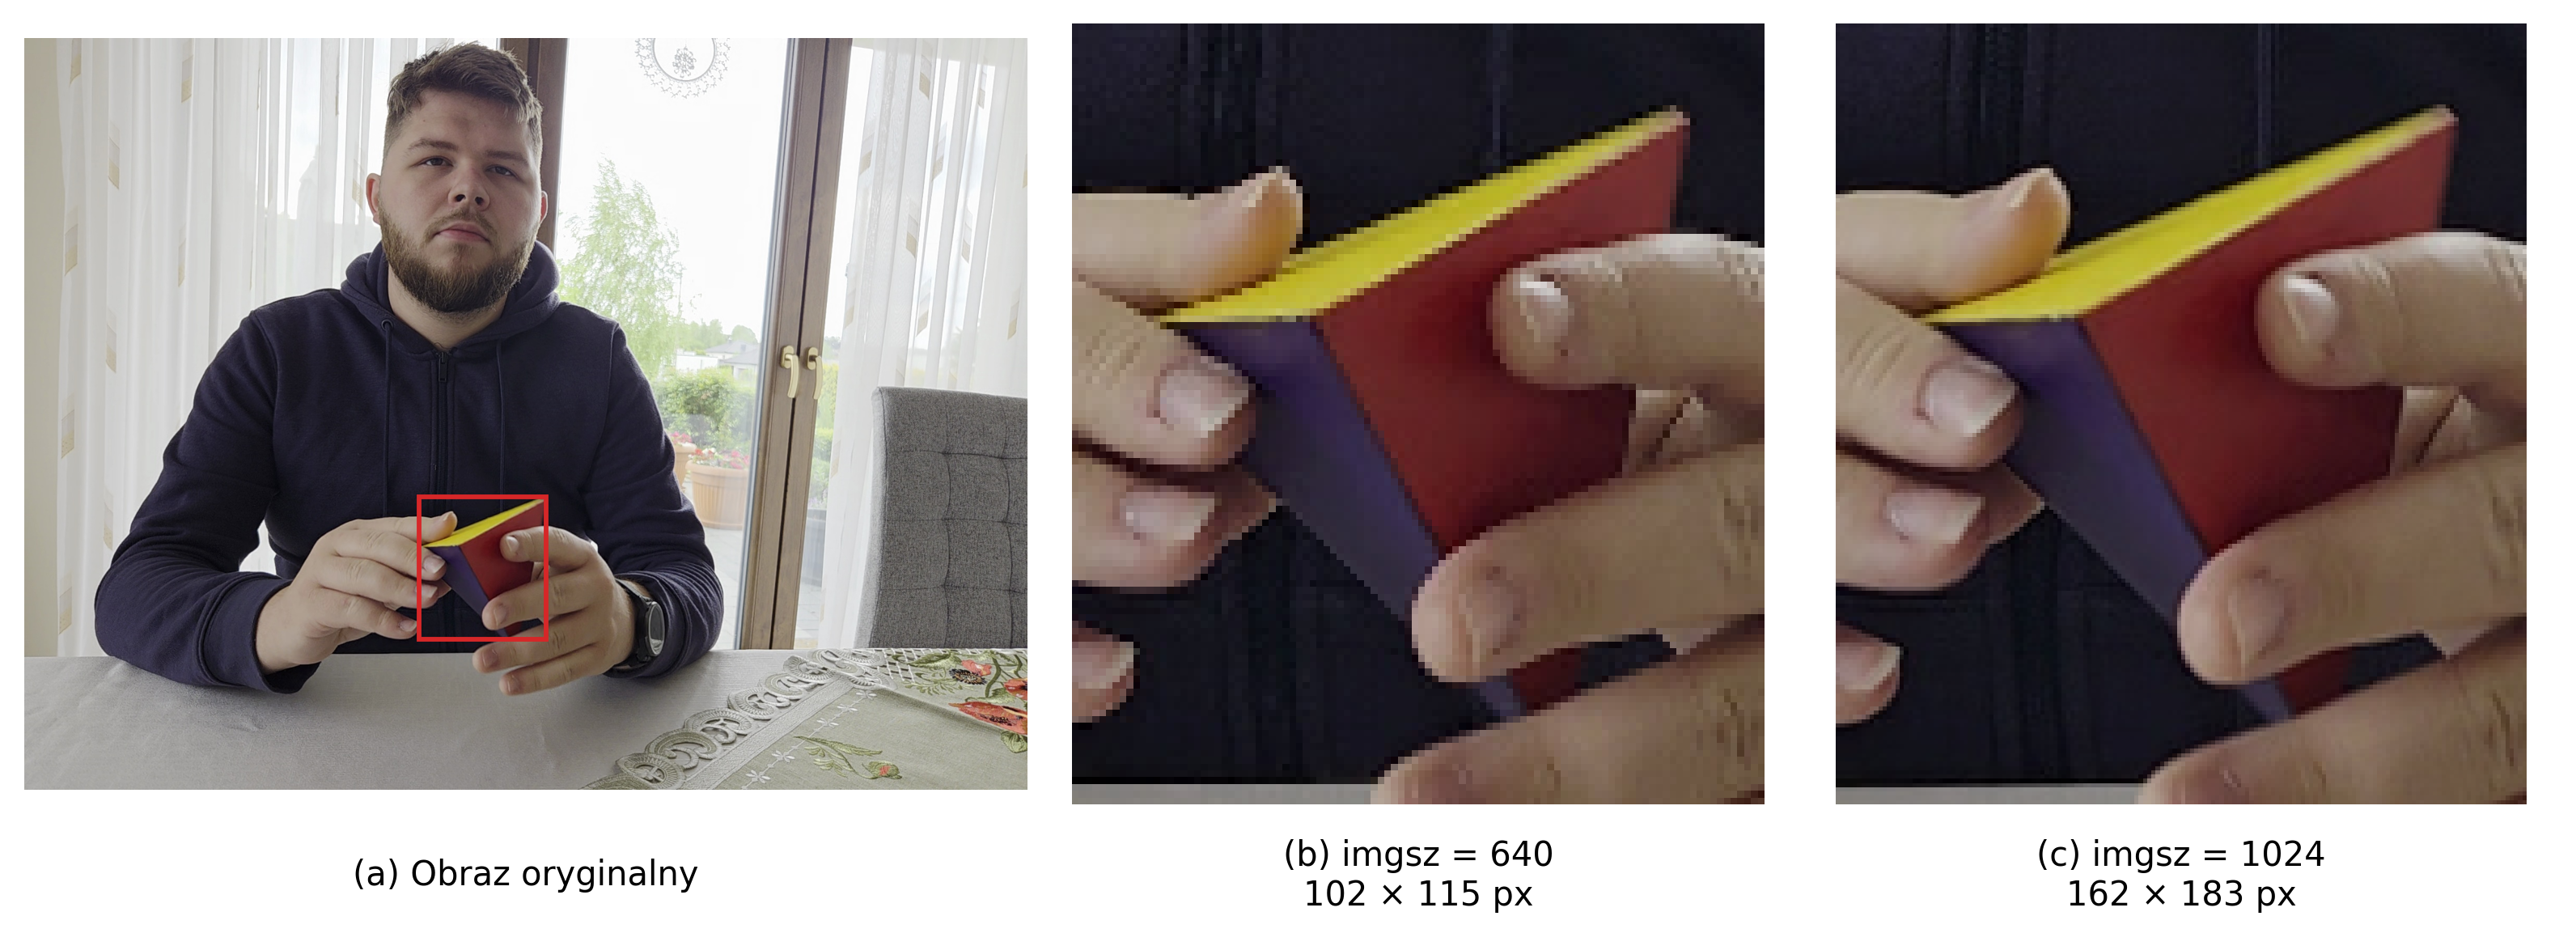
\includegraphics[width=\textwidth]{./graf/img_resize.png}
    \caption{Wizualizacja różnicy rozmiaru obiektu na obrazie w~zależności od rozdzielczości obrazu wejściowego.}
    \label{fig:img_resize}
\end{figure}

Zwiększenie rozdzielczości obrazu wejściowego przyniosło poprawę wszystkich analizowanych wartości metryk dla obu wariantów modeli. Największe zmiany można zauważyć w~przypadku YOLO26n. Wartość metryki $mAP50$ wzrosła o~$14,64$ p.p., a~$mAP50\text{-}95$ o~około $12$ p.p. Jednocześnie wskaźnik $F1$-score wzrósł o~$11,34$ p.p. Wyniki te wskazują na wyraźny wzrost jakości detekcji wraz z~zwiększeniem szczegółowości obrazu wejściowego poprzez zmianę jego rozdzielczości.

Poprawa występuje również dla wariantu \texttt{s}, jednak nie osiąga ona takiego poziomu jak w~przypadku YOLO26n. Zwiększenie rozmiaru wejścia do 1024 pikseli podniosło wartość $mAP50$ o~$5,86$ p.p., $mAP50\text{-}95$ o~$8,81$ p.p., a~$F1$-score o~$5,67$ p.p. W~przeciwieństwie do wariantu \texttt{n}, największy wzrost obserwuje się w~przypadku bardziej rygorystycznej metryki~$mAP50\text{-}95$.

Wyniki porównań pokazują, że rozmiar obrazu wejściowego ma istotny wpływ na jakość detekcji. Zależność jest szczególnie widoczna dla YOLO26n, dla którego zwiększenie rozdzielczości przyniosło poprawę wszystkich analizowanych metryk o~ponad $11$ p.p. Może mieć to związek z~większą liczbą pikseli reprezentujących obiekty na obrazie, dzięki czemu zachowywane jest więcej informacji o~ich krawędziach, powierzchniach, cieniach i~innych cechach widocznych na obrazie.

Wyniki eksperymentu B wskazują, że zwiększenie rozmiaru obrazu wejściowego do 1024 pikseli poprawia znacząco jakość detekcji niezależnie od zastosowanej skali modelu. Jednocześnie, konieczność przetworzenia większej ilości danych wejściowych zwiększa koszt obliczeniowy mogąc prowadzić do wydłużenia czasu inferencji. W~przeciwieństwie do eksperymentu A, w~którym zwiększenie modelu nie musiało przynieść korzyści, eksperyment B wykazuje, że zwiększenie rozdzielczości obrazu wejściowego prowadzi do poprawy działania modeli. Ocena przydatności zwiększenia rozdzielczości musi zostać jednak zestawiona z~kosztami obliczeniowymi, jakie nakłada na system przetwarzanie większej ilości~\nobreakdash{danych}.

\section{Wpływ reprezentacji obrazu na jakość detekcji}
\label{ssec:rgb_grayscale}

Największe różnice pomiędzy badanymi modelami wystąpiły w~eksperymencie C, który polegał na usunięciu informacji o~kolorze z~obrazów wejściowych. Przeciwnie do poprzednich eksperymentów, w~tym przypadku porównywano modele o~jednakowej konfiguracji, uczonych na zbiorach danych o~identycznych obrazach i~adnotacjach, ale pracujących w~reprezentacji kolorowej i~w~odcieniach szarości. Do porównania wykorzystano trzy dostępne pary modeli: YOLO26n 640 ($E_1$, $E_5$), YOLO26s 640 ($E_2$, $E_6$) oraz YOLO26n 1024 ($E_3$, $E_7$). Wyniki przedstawiono w~tabeli~\ref{tab:exp_c}.

\begin{table}[ht]
    \centering
    \caption{Porównanie jakości modeli pracujących na obrazach RGB i~w~odcieniach szarości w~eksperymencie C.}
    \label{tab:exp_c}
    \begin{tabular}{l|l|ccc}
        \toprule
        \textbf{Konfiguracja}      &
        \textbf{Reprezentacja}     &
        \textbf{$mAP50$}           &
        \textbf{$mAP50\text{-}95$} &
        \textbf{$F1$-score}                                          \\
        \midrule

        \multirow{3}{*}{YOLO26n 640}
                                   & RGB
                                   & 0.71595   & 0.59866  & 0.69568  \\
                                   & grayscale
                                   & 0.48831   & 0.36001  & 0.52635  \\
                                   & różnica
                                   & -0.22764  & -0.23866 & -0.16933 \\
        \midrule

        \multirow{3}{*}{YOLO26s 640}
                                   & RGB
                                   & 0.78551   & 0.64119  & 0.73041  \\
                                   & grayscale
                                   & 0.55971   & 0.44940  & 0.61526  \\
                                   & różnica
                                   & -0.22581  & -0.19179 & -0.11515 \\
        \midrule

        \multirow{3}{*}{YOLO26n 1024}
                                   & RGB
                                   & 0.86231   & 0.71856  & 0.80908  \\
                                   & grayscale
                                   & 0.62098   & 0.49469  & 0.62426  \\
                                   & różnica
                                   & -0.24133  & -0.22387 & -0.18482 \\
        \bottomrule
    \end{tabular}
\end{table}


Każda para wykazuje spadek skuteczności detekcji dla wszystkich metryk po usunięciu informacji o~kolorze. Największą różnicę odnotowano w~przypadku modelu YOLO26n przy rozmiarze wejściowym 640 pikseli. Wartość $mAP50\text{-}95$ dla tego wariantu spadła o~$23,9$ p.p. osiągając wartość $36\%$. Podobne zachowanie obserwujemy w~przypadku pozostałych par modeli, gdzie spadek wartości wyniósł $19,2$ p.p. dla wariantu YOLO26s 640 oraz $22,4$ p.p. dla wariantu YOLO26n 1024. Tak duże różnice wskazują, że informacja o~kolorze odgrywa istotną rolę w~procesie detekcji.

Silny spadek wartości zauważamy też w~pozostałych metrykach. Spadki wartości $mAP50$ pomiędzy wariantami wahają się od $22,6$ do $24,1$ p.p., a~dla wskaźnika $F1$-score od $11,5$ do $18,5$ p.p. Widzimy tutaj, że usunięcie informacji o~kolorze ma wpływ nie tylko na rozpoznanie klasy obiektu, ale prowadzi do ogólnego pogorszenia skuteczności detekcji we wszystkich badanych przypadkach.

Jednocześnie, modelem najlepiej radzącym sobie w~środowisku, w~którym wykonywana jest detekcja na obrazach w~odcieniach szarości, jest wariant $E_7$, czyli YOLO26n operujące na obrazach o~rozdzielczości 1024 pikseli. Wartość metryki $mAP50\text{-}95$ dla tego wariantu wyniosła $49,5\%$, a~dla pozostałych wariantów $E_5$ i~$E_6$ wyniosła około $36\%$ i~$44,9\%$. Wyniki te zgadzają się z~obserwacjami z~eksperymentu B, zgodnie z~którymi, w~badanym problemie, zwiększenie rozdzielczości skutkuje poprawą jakości detekcji. Nie niweluje to jednak ograniczeń wynikających z~braku informacji o~kolorze, które prowadzą do bardzo dużego spadku zdolności modelu do wykrywania obiektów.

Eksperyment nie pozwala jednoznacznie określić, że modele RGB rozpoznają bryły wyłącznie na podstawie ich koloru. Modele pracujące na odcieniach szarości nadal zachowują zdolność do wykrywania obiektów, choć popełniają więcej błędów. Wskazuje to, że podczas detekcji modele korzystają również z~innych cech wykrywanych obiektów, jak krawędzie, powierzchnie i~wierzchołki. Uzyskane wyniki wskazują jednak, że informacja o~barwie stanowi ważne źródło informacji, a~jej usunięcie prowadzi do znacznego pogorszenia jakości detekcji.

W~kontekście docelowego zastosowania systemu to porównanie jest szczególnie ważne. Zakłada się, że bryły używane w~środowisku docelowym mogą znacznie różnić się kolorystyką od zestawu wykorzystywanego do stworzenia zbioru uczącego. Wariant pracujący w~grayscale ogranicza możliwość korzystania modelu z~informacji o~kolorze, jednakże wyniki eksperymentu C pokazują, że usunięcie kanału koloru prowadzi do znacznego pogorszenia jakości detekcji. Przeprowadzone porównanie nie pozwala stwierdzić, że badane warianty zapewniają odporność na zmiany kolorystyki. Ocena tego podejścia wymaga dalszych badań na zbiorach danych zawierajacych inne obiekty odpowiadające wykrywanym klasom niż te, które zostały użyte do treningu.

Na podstawie wyników można jednoznacznie stwierdzić, że usunięcie informacji barwnej z~obrazów znacznie pogarsza jakość detekcji wszystkich badanych konfiguracji. Najlepszy wariant nie przekroczył wartości $50\%$ dla metryki $mAP50\text{-}95$, co jest wynikiem niesatysfakcjonującym w~kontekście zastosowania systemu w~środowisku docelowym. Wskazuje to jednak, że informacja o~kolorze nie jest niezbędna do wykonania detekcji. Pomimo tego, rozwój modeli pracujących w~odcieniach szarości może stanowić interesującą gałąź badań, szczególnie w~kontekście zmiennych warunków oświetleniowych czy różnorodności kolorystycznej obiektów w~środowisku docelowym.

\section{Porównanie najlepszych konfiguracji}

Przeprowadzone eksperymenty nie pozwoliły na jednoznaczne wyłonienie wariantu modelu, który osiągnąłby najlepsze wyniki we wszystkich analizowanych aspektach. Uwidoczniły jednak znaczące różnice w~skuteczności detekcji, w~zależności od konfiguracji danego modelu. Z~punktu widzenia zastosowania systemu w~środowisku docelowym, sama jakość detekcji nie jest jednak jedynym kryterium wyboru. Ponieważ przetwarzanie obrazu ma odbywać się w~czasie rzeczywistym, istotne są również koszt obliczeniowy oraz czas potrzebny na wykonanie predykcji.

Do końcowego porównania wybrano cztery konfiguracje reprezentujące najważniejsze kompromisy ukazane w~wcześniejszych badaniach: $E_1$, $E_3$, $E_4$ oraz $E_7$. Pomiary czasu inferencji i~liczby klatek na sekundę wykonano na urządzeniu Apple MacBook Air z~procesorem Apple M1 i~8GB pamięci RAM, używając MPS (ang. \english{Metal Performance Shaders}). Zestawienie jakości detekcji i~kosztu obliczeniowego przedstawiono w~tabeli~\ref{tab:best_models}.

\begin{table}[ht]
    \centering
    \caption{Porównanie wybranych konfiguracji modeli pod względem jakości i~kosztu obliczeniowego.}
    \label{tab:best_models}
    \begin{tabular}{l|cccccc}
        \toprule
        \textbf{Konfiguracja}
                                & \textbf{$mAP50\text{-}95$} & \textbf{$F1$-score} & \textbf{L. Param.} & \textbf{GFLOPs} & \textbf{Czas} & \textbf{FPS} \\
        \midrule
        $E_1$: n RGB 640        & 0.59866                    & 0.69568             & 2.51 M             & 5.78            & 16.55ms       & 60.4         \\

        $E_3$: n RGB 1024       & 0.71856                    & 0.80908             & 2.51 M             & 14.80           & 37.72ms       & 26.5         \\

        $E_4$: s RGB 1024       & 0.72932                    & 0.78712             & 9.95 M             & 57.65           & 85.26ms       & 11.7         \\

        $E_7$: n grayscale 1024 & 0.49469                    & 0.62426             & 2.51 M             & 14.80           & 36.15ms       & 27.7         \\
        \bottomrule
    \end{tabular}
\end{table}

Spośród przedstawionych konfiguracji, najwyższą wartość $mAP50\text{-}95$ osiągnął wariant $E_4$, będący modelem YOLO26s pracującym na obrazach kolorowych o~rozdzielczości 1024 pikseli. Jest to jednocześnie największy model, który wymaga najwięcej zasobów obliczeniowych. Bardzo podobne wyniki osiągnął wariant $E_3$, który pracuje na obrazach tej samej rozdzielczości, ale jest mniejszym modelem YOLO26n. Różnica pomiędzy tymi wariantami w~wartości metryki $mAP50\text{-}95$ wyniosła $1,08$ p.p. Oba modele osiągają więc zbliżoną skuteczność detekcji, a~porównanie metryk nie pozwala jednoznacznie wskazać, który z~nich jest lepszy.

Koszt zastosowania większego wariantu jest jednak czynnikiem, który może dyskwalifikować jego użycie w~systemie. Model $E_4$ zawiera około $9,95$ mln parametrów wobec $2,51$ mln znajdujących się w~wariancie $E_3$, a~liczba operacji wynosi odpowiednio $57,65$ GFLOPs wobec $14,80$ GFLOPs. Oznacza to, że użycie wariantu $E_4$ prowadzi do niemal czterokrotnego zwiększenia tych wartości mimo że główną korzyścią jest minimalny wzrost metryki $mAP50\text{-}95$. Nie jest to wystarczający powód, aby wybrać wariant $E_4$ jako najlepszy do zastosowania w~systemie.

Różnice są widoczne również w~czasie predykcji. Wariant $E_3$ jest w~stanie przetworzyć obraz wejściowy w~czasie o~ponad połowę krótszym niż większy model, osiągając możliwość predykcji $26,5$ klatek na sekundę. Warto jednak zaznaczyć, że mierzony czas uwzględnia jedynie działanie mechanizmu predykcji modelu, a~nie czas odpowiedzi systemu. Na ten wpływają również transmisja obrazu, jego dekodowanie i~pozostałe etapy przetwarzania. Zmierzone wartości służą jedynie do porównania modeli uruchomionych w~tych samych~\nobreakdash{warunkach}.

Odmienny kierunek optymalizacji zauważamy w~przypadku wariantu $E_1$, który działa na obrazach o~mniejszej rozdzielczości. Reprezentuje on podejście nastawione przede wszystkim na optymalizację kosztów, przez co osiąga wyniki gorsze od wariantu $E_3$ o~około $12$ p.p. w~metryce $mAP50\text{-}95$. Jednocześnie obniża koszt predykcji do poziomu $5,78$ GFLOPs, co stanowi wartość niemal trzykrotnie mniejszą względem wariantu $E_3$. Wpływa to również na płynniejsze działanie, będąc w~stanie przetworzyć pojedynczy obraz wejściowy w~czasie krótszym niż $17$ ms. Ten wariant może być rozważany w~przypadku jednostek o~bardzo ograniczonej mocy obliczeniowej, jednak nie ukazuje tak dobrego kompromisu pomiędzy skutecznością detekcji a~kosztem obliczeniowym.

Osobną rolę w~porównaniu stanowi model $E_7$ pracujący na obrazach w~odcieniach szarości. Jest on najlepszym spośród trzech wariantów wykorzystujących dodatkowy filtr przekształcający obrazy. Jego koszt obliczeniowy pozostaje zbliżony do wariantu $E_3$ -- oba wykorzystują tę samą architekturę i~ten sam rozmiar obrazu wejściowego. Znacznie niższa skuteczność detekcji w~porównaniu do pozostałych wariantów jest jednak istotnym ograniczeniem, które może dyskwalifikować go w~zastosowaniach wymagających wysokiej skuteczności detekcji. Może jednak stanowić istotny punkt odniesienia przy dalszych badaniach nad zależnością detekcji od informacji o~barwie.

Z~punktu widzenia kompromisu pomiędzy skutecznością a~kosztem obliczeniowym, najkorzystniejszym wariantem pozostaje konfiguracja $E_3$: YOLO26n pracujący na obrazach kolorowych o~rozdzielczości 1024 pikseli. Osiąga on gorsze wartości metryki $mAP50\text{-}95$, jednocześnie osiągając lepsze wartości wskaźnika $F1$-score niż wariant $E_4$. Jednocześnie jest od niego znacznie szybszy i~powinien być pierwszym wyborem do zastosowania w~systemie. W~badaniach dodatkowy koszt wynikający z~użycia wariantu YOLO26s nie przynosi poprawy jakości wystarczającej do uzasadnienia wyboru większego wariantu jako podstawowego modelu systemu.

\section{Analiza błędów detekcji}

Globalne wartości $mAP$ i~$F1$-score pozwalają wykonać ogólną ocenę skuteczności modeli, jednakże nie ukazują one szczegółowego obrazu błędów popełnianych przez system. Dlatego, w~celu ich dokładniejszego określenia należy przyjrzeć się macierzom pomyłek, które zostały uzyskane podczas pracy modeli na zbiorze testowym. Wybrano te same cztery konfiguracje, które zostały poddane ocenie w~poprzedniej sekcji. Za punkt odniesienia przyjęto wariant $E_3$, który został wskazany jako najkorzystniejszy pod względem ocenianego kompromisu. Pozostałe warianty pozwalają natomiast ocenić, w~jaki sposób zmienia się charakter błędów w~zależności od czynników treningu.

Znormalizowane macierze pomyłek ukazują procentowy udział predykcji modelu. Mocno zarysowana główna przekątna wskazuje, że model poprawnie klasyfikuje większość obiektów, a~wartości poza nią wskazują na błędy detekcji. Kolumny macierzy odpowiadają rzeczywistym klasom obiektów, natomiast wiersze klasom przewidywanym przez model. Wiersz \english{background} oznacza przypadki, w~których model nie wykrył żadnego obiektu, a~kolumna \english{background} przypadki, w~których na obrazie nie było żadnego obiektu. Macierze analizowanych modeli przedstawiono na rysunku~\ref{fig:confusion_matrices}.

\begin{figure}[htbp!]
    \centering
    \begin{subfigure}{\textwidth}
        \centering
        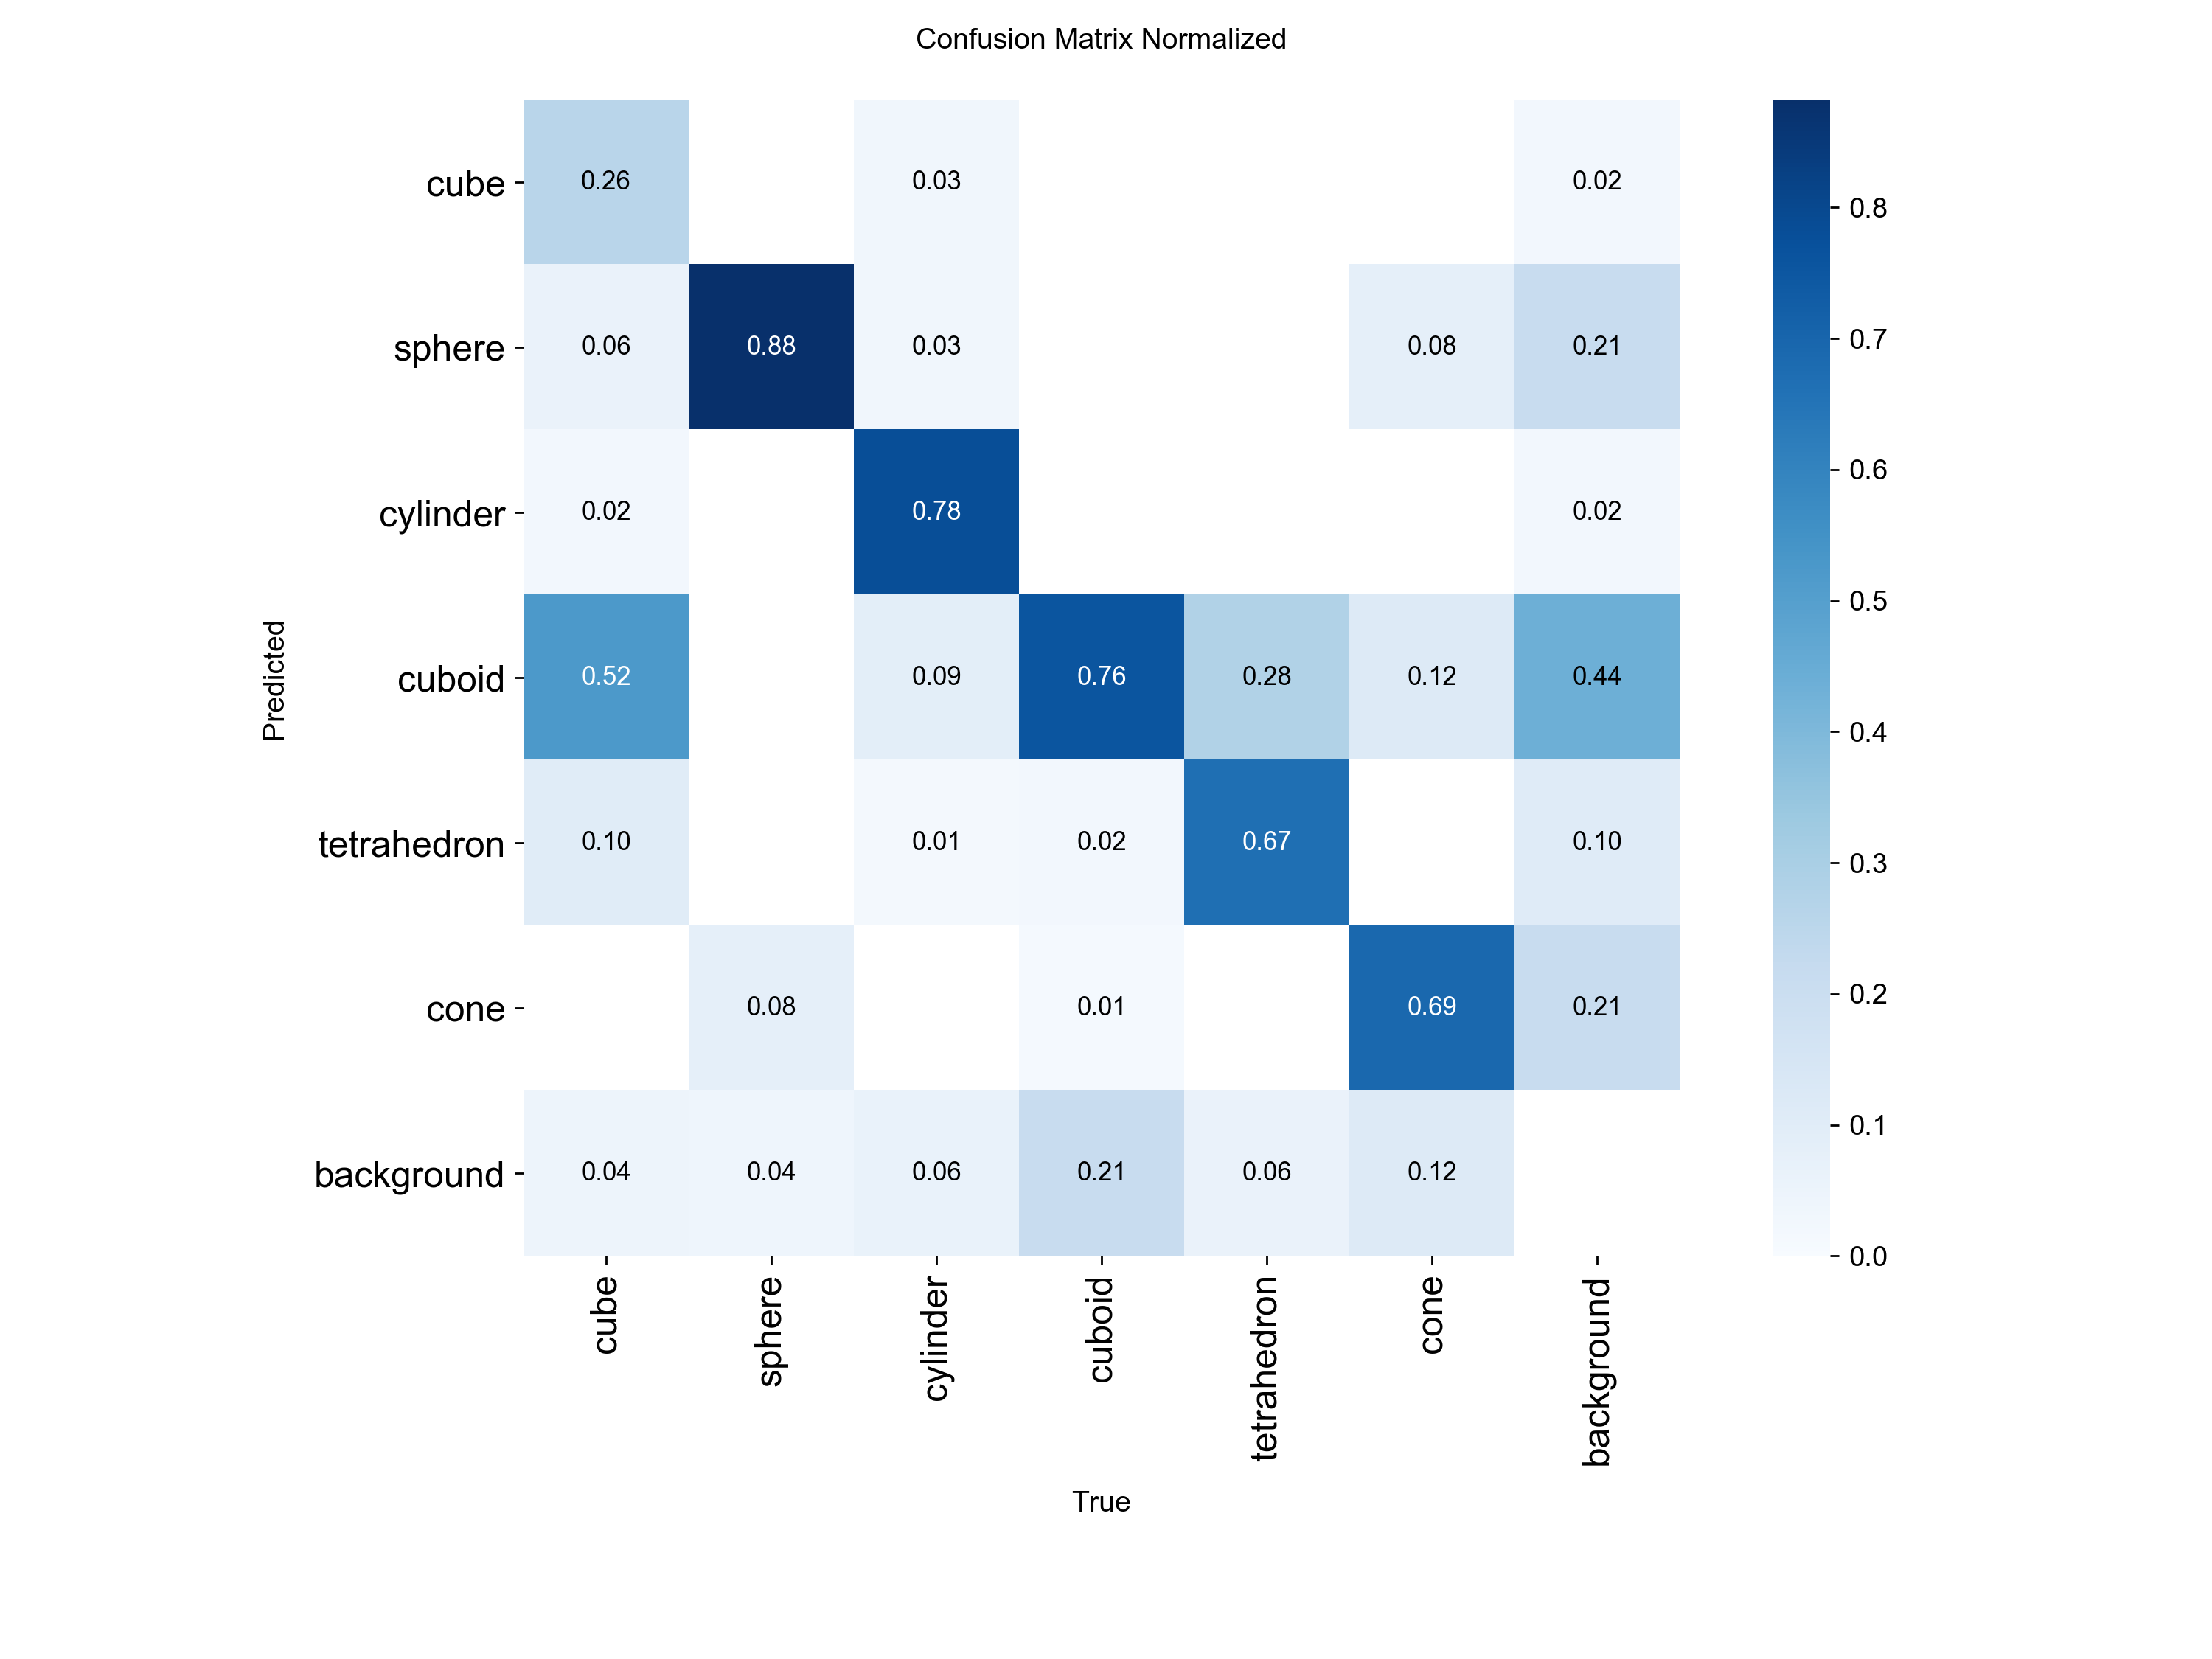
\includegraphics[width=0.9\textwidth]{./graf/conf_matrix/E1.png}
        \caption{Wariant $E_1$: YOLO26n 640 RGB.}
        \label{fig:confusion_matrix_e1}
    \end{subfigure}
    \hfill
    \begin{subfigure}{\textwidth}
        \centering
        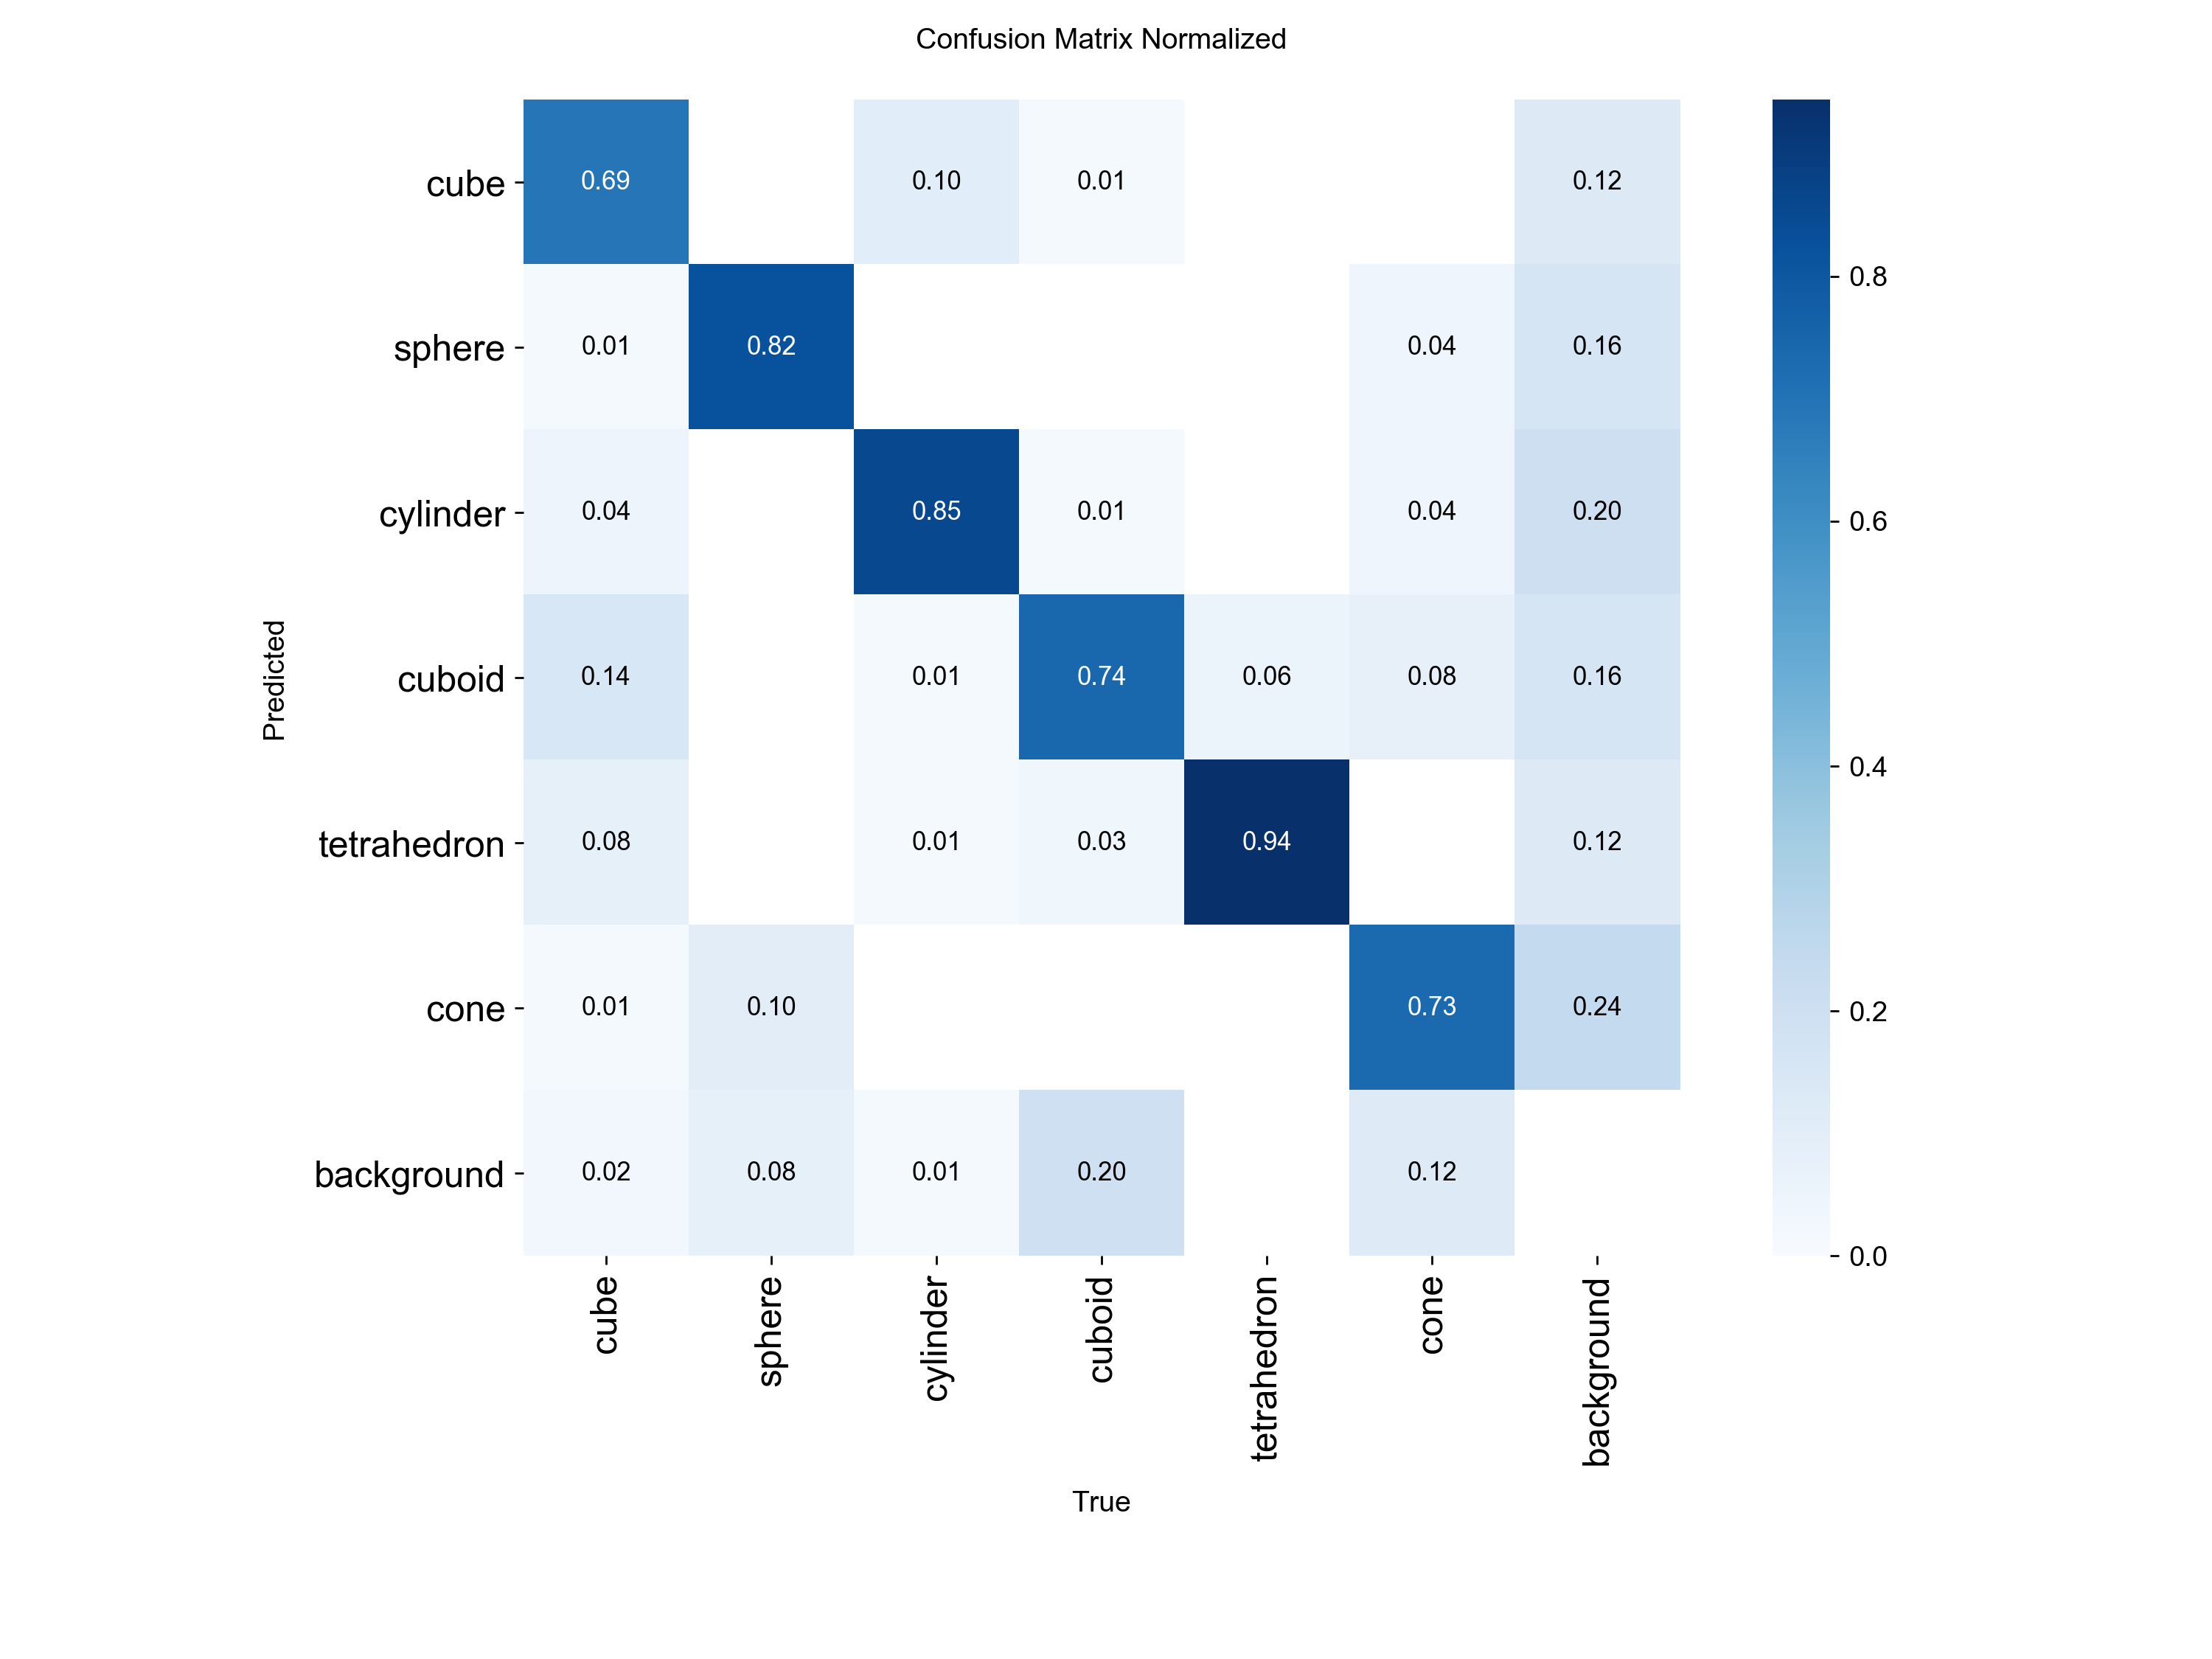
\includegraphics[width=0.9\textwidth]{./graf/conf_matrix/E3.png}
        \caption{Wariant $E_3$: YOLO26n 1024 RGB.}
        \label{fig:confusion_matrix_e3}
    \end{subfigure}
\end{figure}
\begin{figure}[htbp!]
    \ContinuedFloat\centering
    \begin{subfigure}{\textwidth}
        \centering
        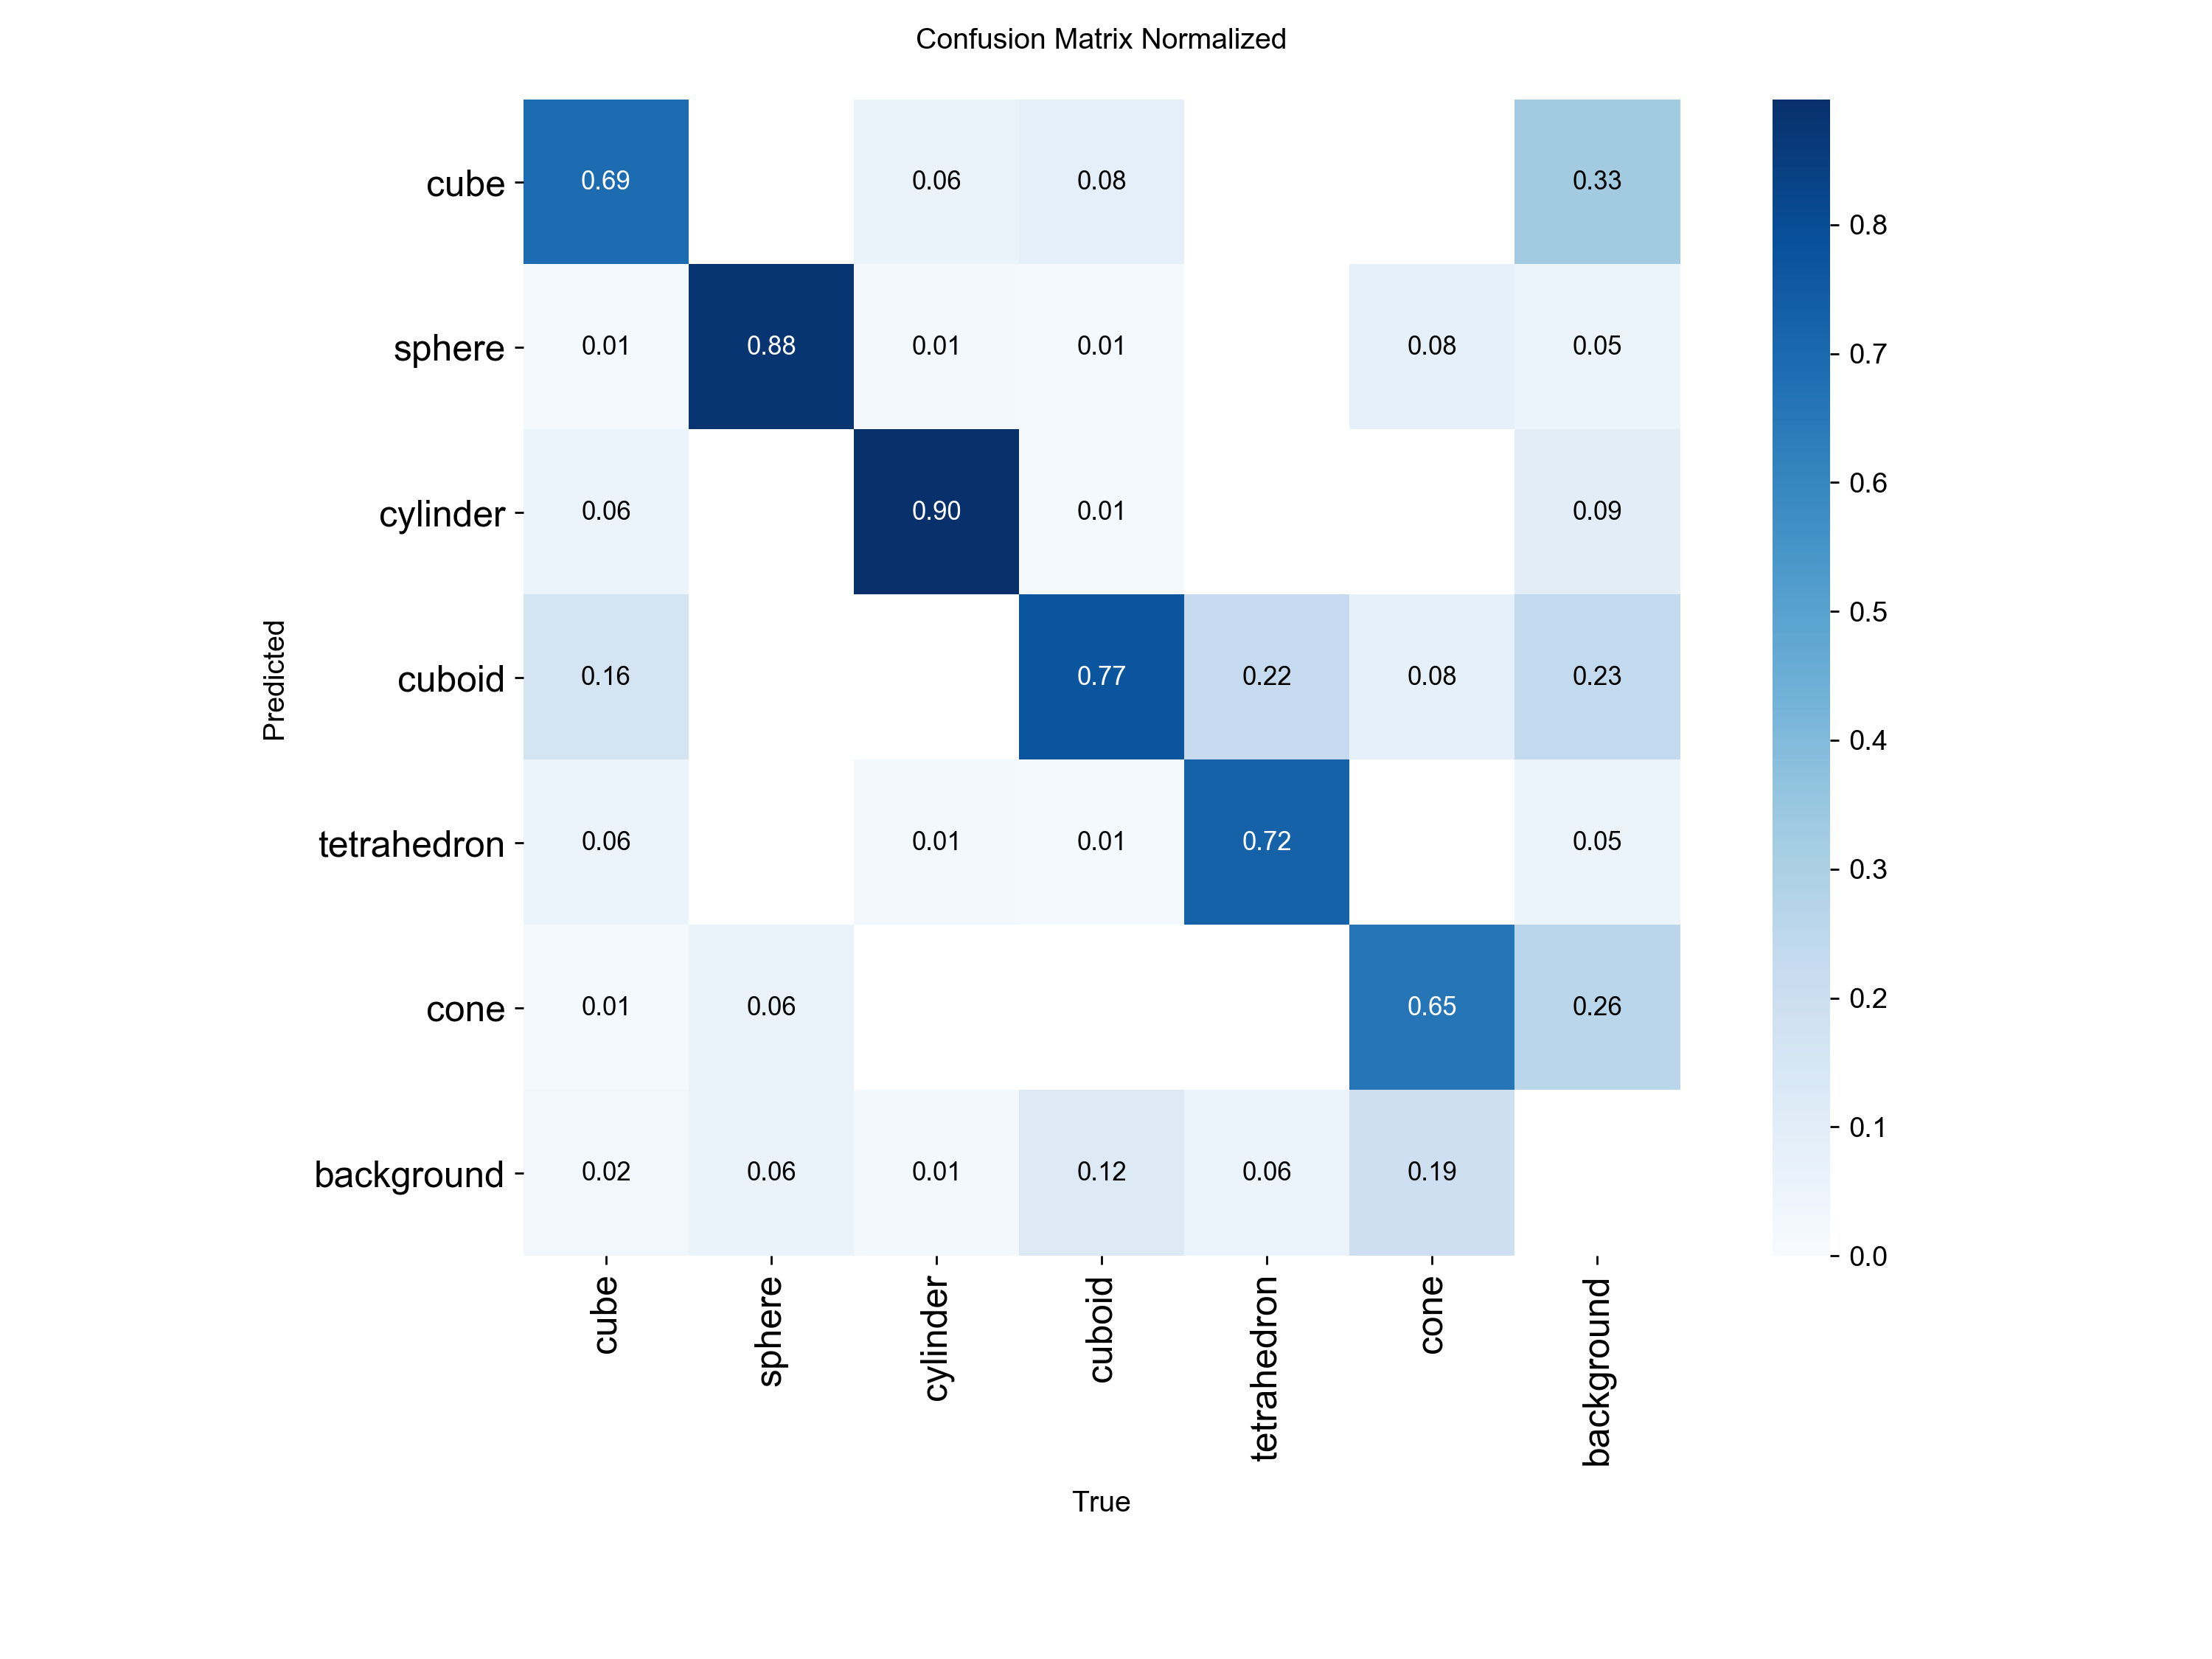
\includegraphics[width=0.9\textwidth]{./graf/conf_matrix/E4.png}
        \caption{Wariant $E_4$: YOLO26s 1024 RGB.}
        \label{fig:confusion_matrix_e4}
    \end{subfigure}
    \hfill
    \begin{subfigure}{\textwidth}
        \centering
        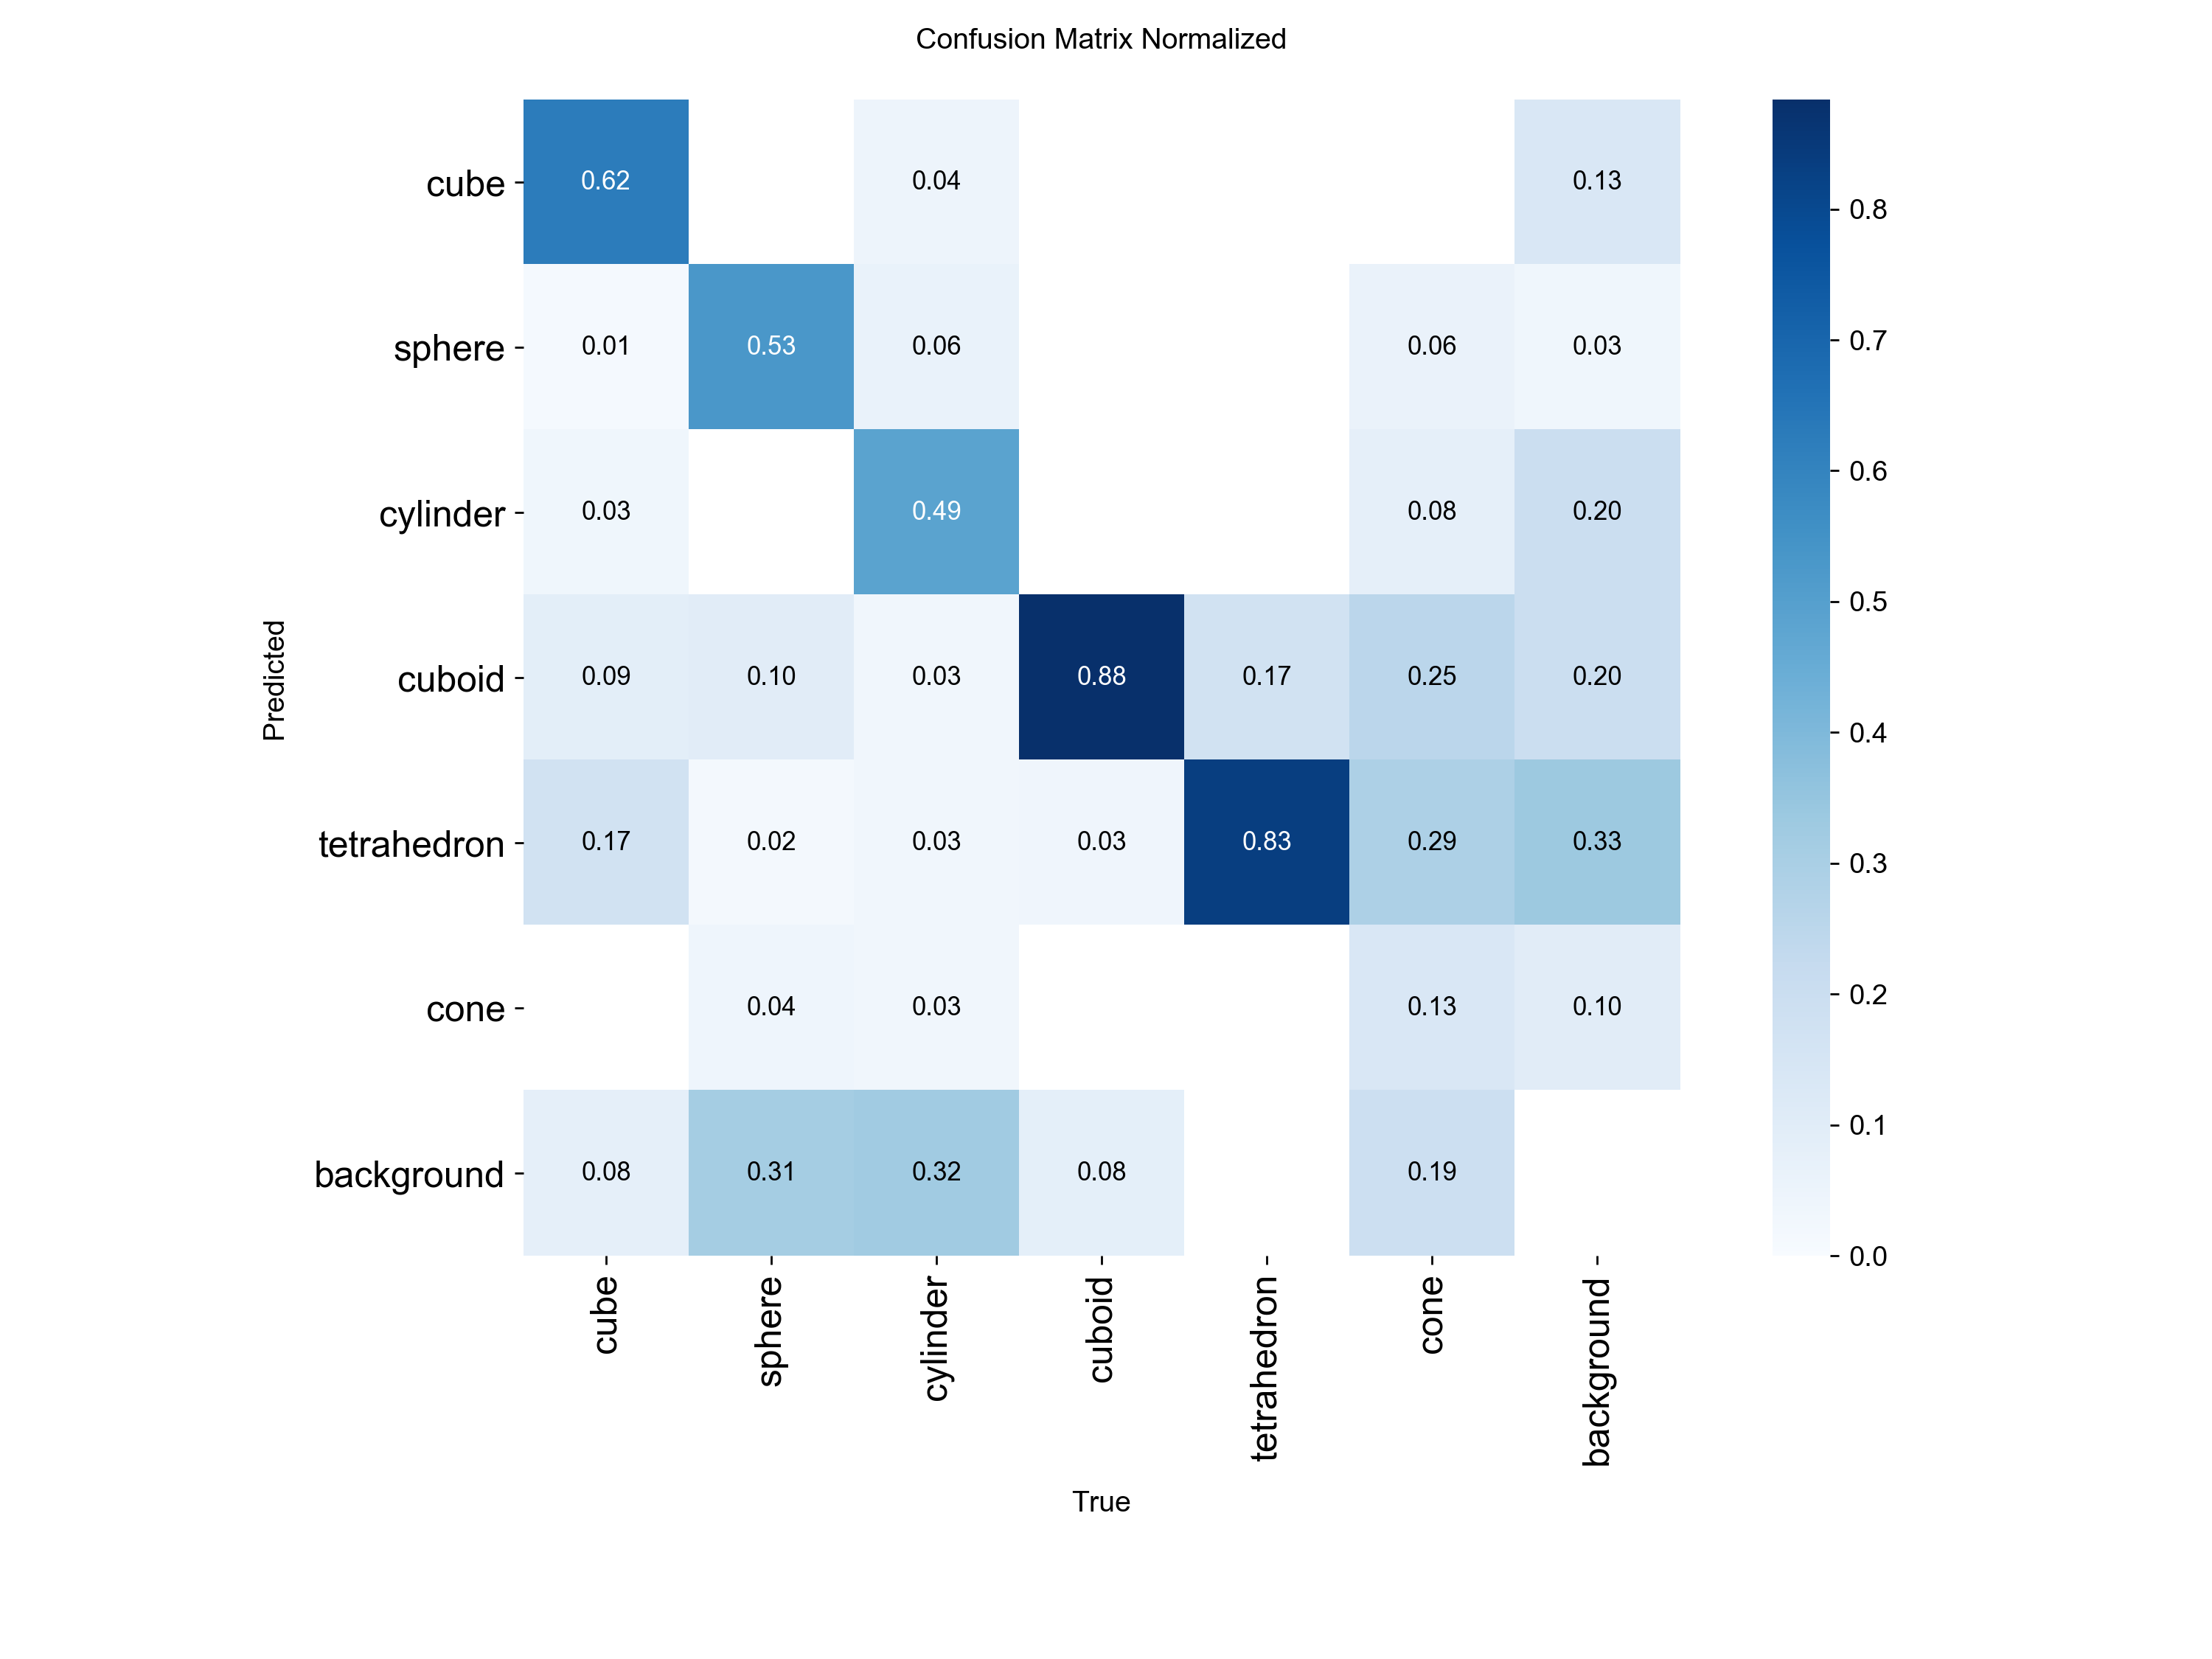
\includegraphics[width=0.9\textwidth]{./graf/conf_matrix/E7.png}
        \caption{Wariant $E_7$: YOLO26n 1024 grayscale.}
        \label{fig:confusion_matrix_e7}
    \end{subfigure}

    \caption{Wybrane znormalizowane macierze pomyłek badanych modeli.}
    \label{fig:confusion_matrices}
\end{figure}

Szczególnie wyraźną różnicę zauważyć można porównując modele $E_1$ i~$E_3$, które różnią się jedynie rozmiarem obrazu wejściowego. Pierwszy z~nich ma problemy z~wykrywaniem sześcianów, które bardzo często klasyfikuje jako prostopadłościany. Poprawnie sklasyfikowano jedynie $26\%$ z~nich, a~ponad połowa została przypisana do klasy prostopadłościanów. Zauważamy też, że model często znajduje prostopadłościany w~miejscach, w~których ich nie ma, co może wskazywać na ich nadmierne przypisywanie obiektów do tej klasy. Zwiększenie rozmiaru obrazu wejściowego w~wariancie $E_3$ znacznie poprawiło skuteczność odróżnienia sześcianów od prostopadłościanów, co może wynikać z~zachowania większej ilości szczegółów obrazu, ułatwiających rozróżnienie proporcji, ścian i~krawędzi obu brył.

Podobne zachowanie obserwujemy dla innych klas. Zwiększenie rozdzielczości skutkuje wzrostem poprawnych klasyfikacji z~$78\%$ do $85\%$ dla walca i~z~$67\%$ do $94\%$ dla czworościanu. Nie wszystkie klasy jednak reagują w~ten sam sposób -- dla kuli ilość poprawnych predykcji spada o~$6$ punktów procentowych, a~dla prostopadłościanu pozostaje na zbliżonym poziomie. Te wyniki uzupełniają wnioski płynące z~eksperymentu~B: zwiększenie rozdzielczości obrazu poprawia globalną zdolność modelu do wykrywania obiektów, ale nie dla każdej klasy osobno.

Przy zestawieniu modeli $E_3$ i~$E_4$ widzimy zgoła inny obraz. Zwiększenie skali modelu poprawia udział poprawnych detekcji dla kuli, walca i~prostopadłościanu, ale osiąga znacząco gorsze wyniki dla czworościanu i~stożka. Dla pierwszego z~nich ilość poprawnych detekcji spada o~$22$ punkty procentowe, a~dla drugiego o~$8$ punktów procentowych. Niewielka przewaga w~$mAP50\text{-}95$ wariantu $E_4$ nie wynika więc z~równomiernej poprawy detekcji wszystkich klas, a~raczej z~ograniczenia części błędów. Jednocześnie, większy model popełnia więcej błędów w~innych przypadkach, co stanowi kolejny argument za wyborem wariantu $E_3$ do zastosowania w~systemie.

Największą zmianę w~charakterze i~ilości błędów detekcji obserwujemy w~przypadku wariantu $E_7$, korzystającego z~obrazów w~odcieniach szarości. Usunięcie informacji o~kolorze nie wpływa równomiernie na zdolność rozpoznawania poszczególnych klas. Na wysokim poziomie pozostaje wykrywanie prostopadłościanów i~czworościanów, osiągając wyniki powyżej $83\%$. W~porównaniu z~modelem $E_3$ zdecydowanie gorzej radzi sobie z~wykrywaniem kuli i~walca -- w~obu przypadkach spadek wyniósł ponad $29$ punktów procentowych. Najgorszy wynik został zanotowany dla klasy stożka, którego poprawne wykrycie odbyło się tylko w~$13\%$ przypadków, a~$29\%$ z~nich zostało sklasyfikowane jako czworościany. Wskazuje to, że usunięcie informacji o~barwie szczególnie wpływa na zdolność modelu do rozróżniania tej klasy od innych.

Model pracujący na obrazach w~odcieniach szarości wykazuje również większą liczbę pominiętych obiektów. Wiersz \english{background} macierzy odpowiada obiektom referencyjnym, do których nie dopasowano żadnej predykcji. Dla modelu $E_7$ udział takich przypadków wynosi $31\%$ dla kuli i~$32\%$ dla walca, podczas gdy model $E_3$ wartości te osiągają odpowiednio $8\%$ i~$1\%$. Dla pozostałych klas wyniki pozostają na zbliżonym poziomie. Pogorszenie wyników wynika więc nie tylko z~błędnego przypisania klas, ale również ze zwiększonej liczby niewykrytych obiektów.

Macierze pomyłek nie są jednak jedynym źródłem informacji o~błędach detekcji. Warto również przyjrzeć się krzywym precyzji i~czułości, które pozwalają ocenić jak zmienia się kompromis pomiędzy tymi dwoma metrykami w~zależności od progu decyzyjnego. Z~tego względu analizę uzupełniono o~wykresy krzywych precision--recall. Na rysunku~\ref{fig:pr_curves} zestawiono je dla wariantów $E_3$ oraz $E_7$. Reprezentują one wybraną konfigurację docelową oraz wpływ ograniczenia koloru na jakość detekcji.

\begin{figure}[htbp!]
    \centering
    \begin{subfigure}{\textwidth}
        \centering
        
\includegraphics[width=\textwidth]{./graf/pr_curve/E3.png}
        \caption{Wariant $E_3$: YOLO26n 1024 RGB.}
        \label{fig:pr_curve_e3}
    \end{subfigure}
    \begin{subfigure}{\textwidth}
        \centering
        
\includegraphics[width=\textwidth]{./graf/pr_curve/E7.png}
        \caption{Wariant $E_7$: YOLO26n 1024 grayscale.}
        \label{fig:pr_curve_e7}
    \end{subfigure}

    \caption{Krzywe precision--recall modeli $E_3$ i~$E_7$ uzyskane na zbiorze testowym.}
    \label{fig:pr_curves}
\end{figure}

Krzywe PR umożliwiają ocenę, w~jaki sposób wzrost czułości oddziałuje na precyzję detekcji poszczególnych klas. Ich przebieg ukazuje rozwinięcie informacji przekazywanych przez metryki AP i~$mAP$, ponieważ pozwala ocenić zachowanie modelu w~całym zakresie kompromisu pomiędzy tymi dwoma metrykami. Porównanie wariantów $E_3$ i~$E_7$ pozwala sprawdzić, czy pogorszenie jakości spowodowane usunięciem informacji o~kolorze dotyczy pojedynczego progu działania, czy też jest widoczne w~szerszym zakresie pracy modelu.

Dla modelu $E_3$ średnia wartość AP przy progu IoU równym $0,5$ wyniosła $0,862$. Najwyższe wartości uzyskano dla klas kuli i~walca, które osiągnęły wartości powyżej $0,94$, a~także dla sześcianu, którego AP50 wyniosło $0,875$. Najsłabszym wynikiem spośród wszystkich klas charakteryzuje się prostopadłościan, dla którego wartość wyniosła $0,732$. Mimo obserwowanej na macierzach pomyłek tendencji do mylenia sześcianów z~prostopadłościanami, model prezentuje wysoką precyzję dla większości klas, również po zwiększeniu progu czułości.

Znacznie bardziej zróżnicowany przebieg krzywych PR obserwujemy w~przypadku wariantu $E_7$. W~jego przypadku $mAP50$ spada do wartości $0,621$. Model osiąga najwyższe wyniki dla prostopadłościanu i~sześcianu, dla których wartości AP50 są powyżej $0,84$, pozostając zbliżonymi do modelu pracującego w~przestrzeni kolorowej. Pozostałe klasy osiągają jednak znacznie niższe wyniki. Najniższe wartości uzyskano dla stożka i~czworościanu, dla których AP50 wyniosło około $0,41$. Ma to swoje odzwierciedlenie w~macierzy pomyłek, w~której widać, że model ma największe problemy z~wykrywaniem stożków.

Porównanie krzywych pochodzących z~tych dwóch modeli potwierdza więc, że pogorszenie wyników po usunięciu informacji o~kolorze nie jest ograniczone do jednego progu czułości, a~dotyczy całego zakresu pracy modelu. Różnice utrzymują się w~szerokim zakresie kompromisu, a~ich wielkość jest silnie zależna od klasy obiektu. Szczególnie istotny jest fakt, że oba modele zachowują wysokie wartości AP50 dla sześcianu i~prostopadłościanu niezależnie od wykorzystania koloru do detekcji. Niestety, dla pozostałych klas wartość ta ulega znacznemu pogorszeniu. Wskazuje to, że model wykorzystuje informacje o~kolorze w~procesie detekcji, lecz jego znaczenie nie jest jednakowe dla wszystkich klas.

Poza zależnościami precision-recall z~punktu widzenia systemu istotny jest również wybór progu pewności predykcji. Jego zbyt niskie ustawienie może zwiększyć liczbę wykrywanych obiektów, jednak może również prowadzić do zwiększenia ilości fałszywych predykcji. Z~drugiej strony, zbyt rygorystyczne ustawienie progu ograniczy udział błędnych wskazań kosztem pominięcia części obiektów. Wybór optymalnej wartości progu, w~którym zachowany jest najlepszy kompromis pomiędzy precyzją a~czułością, może zostać dokonany na podstawie krzywej $F1$. Zależność $F1$-score od progu pewności predykcji dla wariantu $E_3$ przedstawiono na rysunku~\ref{fig:f1_curve_e3}.

\begin{figure}[ht]
    \centering
    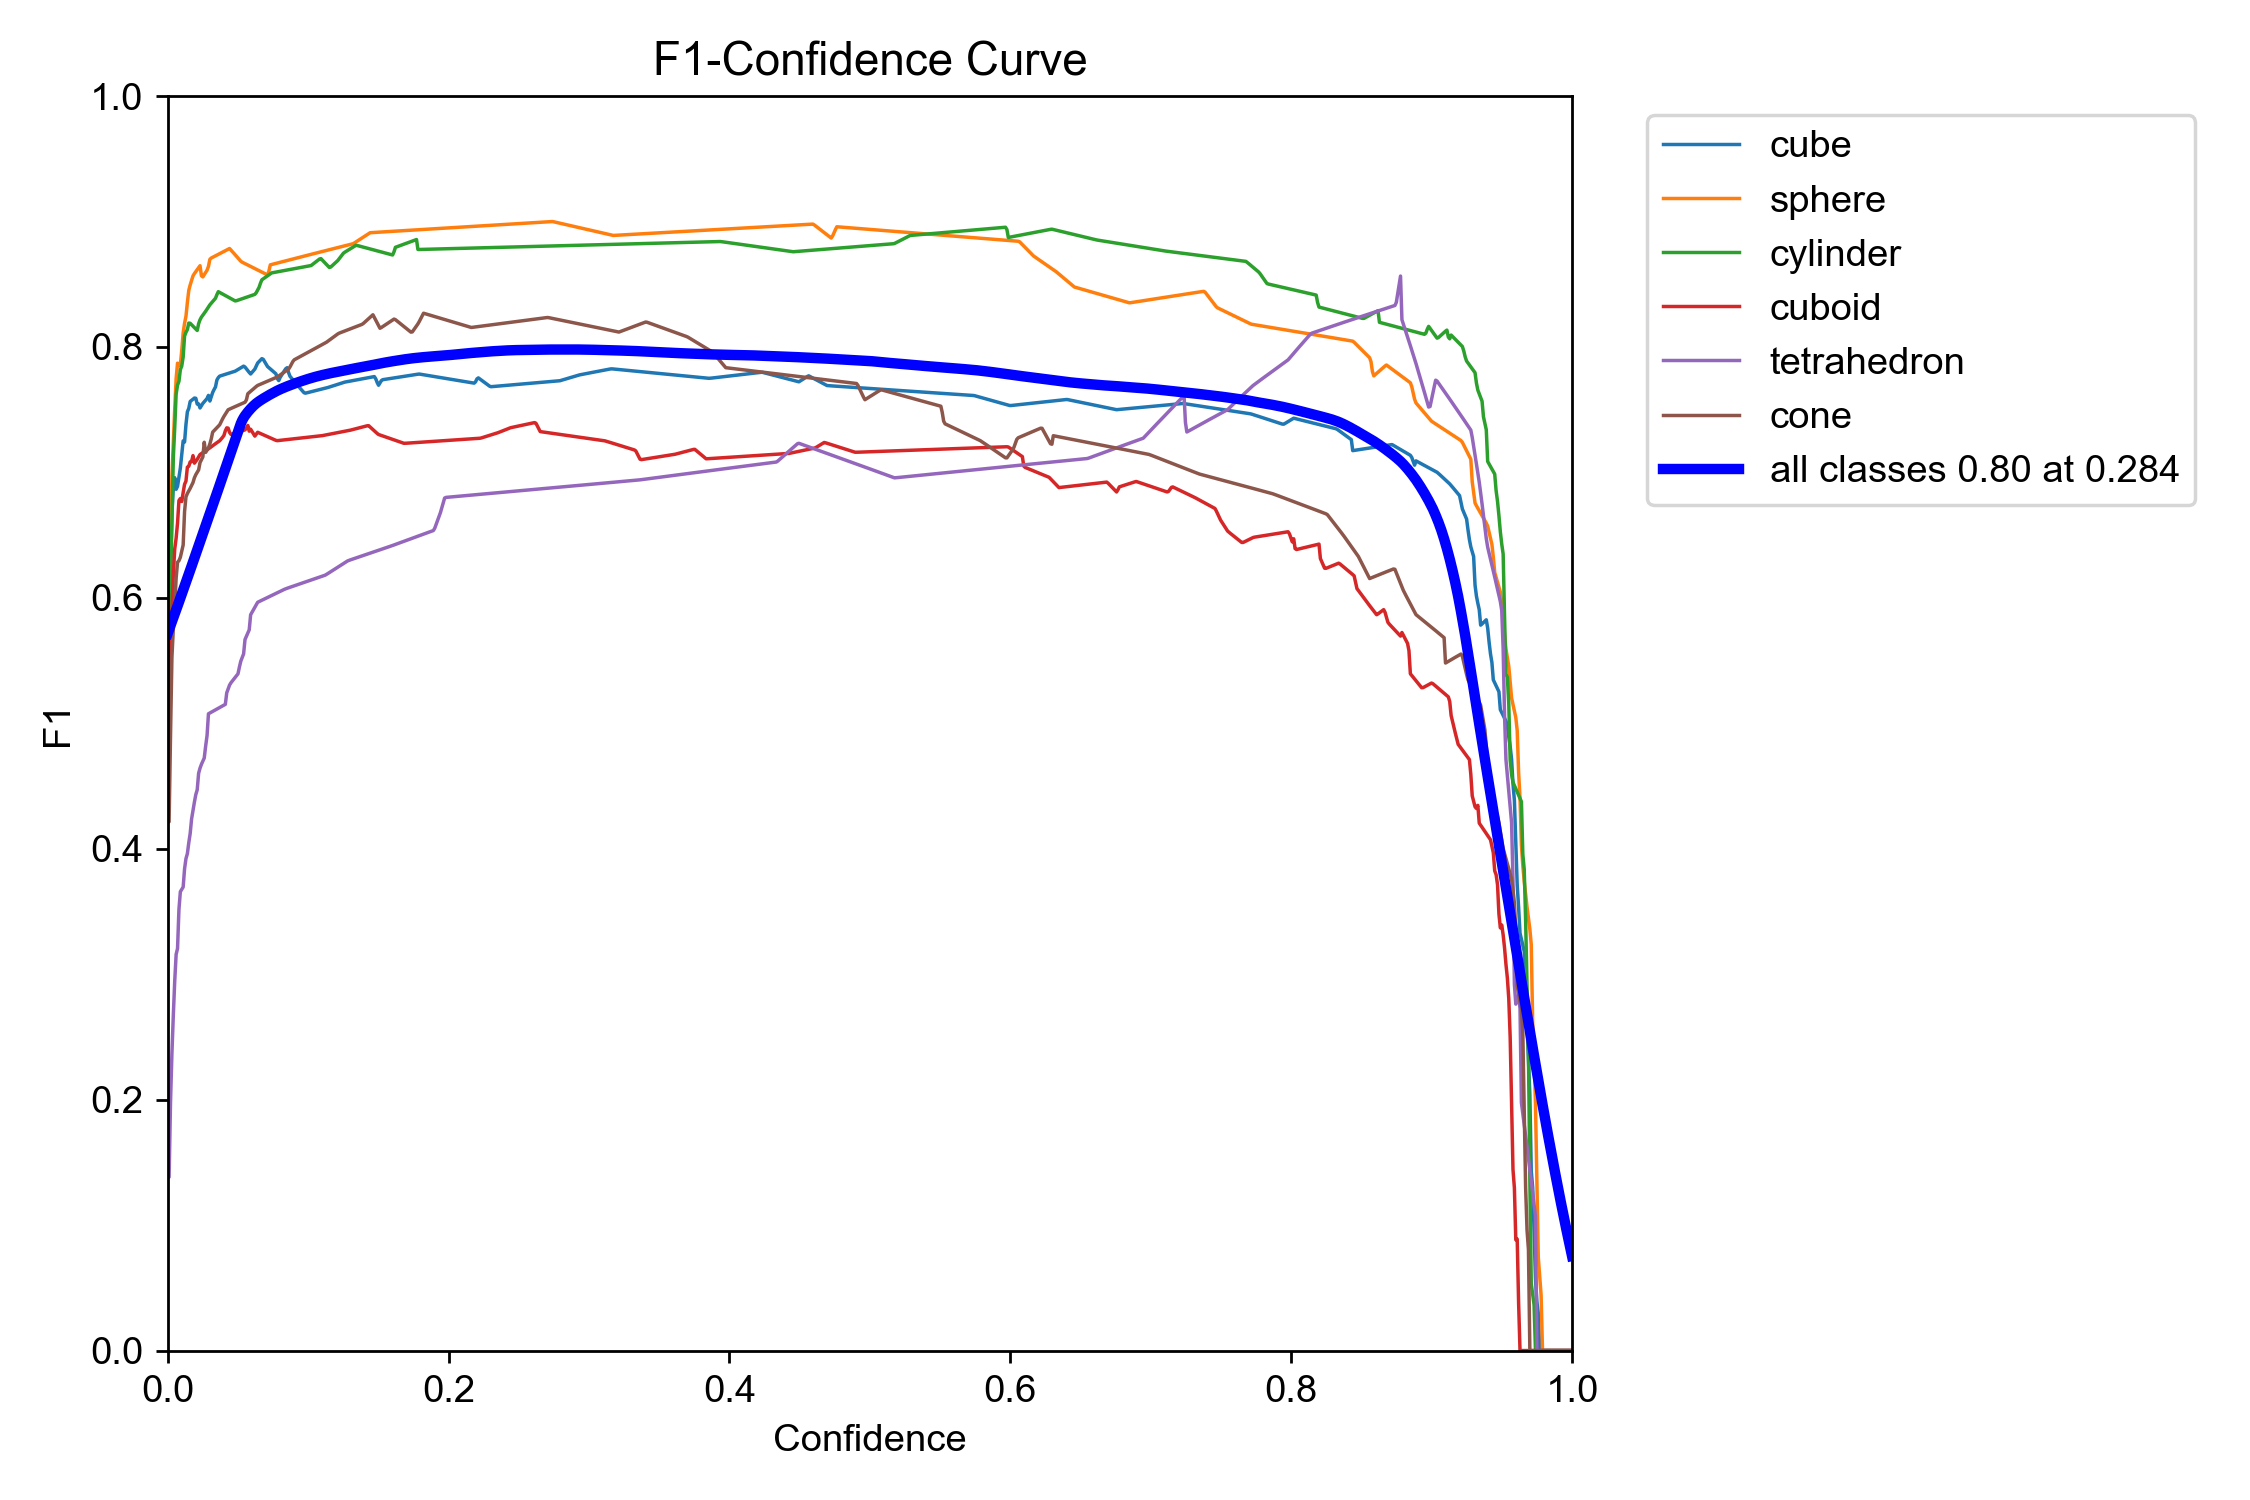
\includegraphics[width=0.9\textwidth]{./graf/E3_F1_curve.png}
    \caption{Krzywa $F1$ dla wariantu $E_3$.}
    \label{fig:f1_curve_e3}
\end{figure}

Dobór odpowiedniej wartości progu jest szczególnie ważny w~kontekście docelowego systemu, ponieważ wpływa on bezpośrednio na to, które detekcje zostaną uznane za wystarczająco pewne i~przekazane do dalszego przetwarzania. Wynik benchmarku jakościowego może więc posłużyć nie tylko do porównania modeli, ale przede wszystkim do doboru parametrów pracy wybranego modelu $E_3$ w~systemie docelowym.

Dla modelu YOLO26n 1024 RGB, który został wskazany jako wariant docelowy, najwyższa wartość krzywej $F1$ jest osiągana przy progu pewności predykcji równym około $0,284$ i~wynosi około $0,8$. W~tym obszarze zachowany jest najlepszy kompromis precyzji i~czułości. Przy zwiększaniu progu możemy zauważyć stopniowy spadek wartości wskaźnika, a~wysokie wartości pewności -- powyżej $0,9$ -- prowadzą do załamania się krzywej i~nagłego spadku wartości $F1$-score. Wartość progu około $0,284$ może więc zostać przyjęta jako punkt odniesienia przy konfiguracji systemu docelowego, ale nie należy jej traktować jako wartości ostatecznej. Koszty poniesione przez błędne detekcje i~pominięte obiekty nie muszą być jednakowe w~każdym przypadku, dlatego ostateczny próg powinien zostać dobrany zależnie od oczekiwanego działania systemu. W~szczególności zasadne może być jego zwiększenie celem ograniczenia błędnych informacji przekazywanych użytkownikowi końcowemu, kosztem częstszego pomijania obiektów.

Analiza macierzy pomyłek i~krzywych pokazuje, że różnice poszczególnych modeli nie sprowadzają się wyłącznie do zmian parametrów i~wartości metryk globalnych. Poszczególne zmiany wpływają na charakter i~częstość popełnianych błędów. Zwiększenie rozdzielczości obrazu wejściowego w~największym stopniu ułatwiło modelowi odróżnienie sześcianów od prostopadłościanów, a~zwiększenie skali modelu poprawiło wyniki tylko części klas. Największy wpływ miało usunięcie informacji o~kolorze, ale ono również nie wpłynęło równomiernie na wszystkie klasy. Zdolność rozpoznawania sześcianu i~prostopadłościanu pozostała na wysokim poziomie.

Podczas interpretacji wyników należy jednak pamiętać, że w~zbiorze testowym nie występowała równa liczba klas obiektów. W~przypadku klas reprezentowanych przez małą liczbę obiektów, pojedynczy błąd może mieć znaczący wpływ na wartości widoczne w~znormalizowanej macierzy. Takie zachowanie można zaobserwować w~przypadku klasy czworościanu, która występowała w~zbiorze testowym jedynie $18$ razy. Z~tego względu nie należy wyciągać zbyt daleko idących wniosków na podstawie różnic obserwowanych w~przypadku tej klasy ani formułować wniosków o~statystycznie istotnych różnicach w~skuteczności~\nobreakdash{detekcji}.

Macierze pomyłek i~krzywe PR nie stanowią również pełnego przeglądu wszystkich aspektów detekcji. Model może poprawnie wskazywać klasę obiektu, ale nieprawidłowo określać jego położenie. Taki błąd będzie widoczny w~metryce $mAP50\text{-}95$, ale nie musi być odzwierciedlony w~analizie klas. Z~tego powodu wyniki przedstawione w~tej sekcji należy rozpatrywać łącznie z~wynikami metryk globalnych oraz z~porównaniem wydajności modeli. Dopiero w~ten sposób możliwe jest uzyskanie pełnego obrazu skuteczności detekcji i~charakteru popełnianych błędów.

\section{Dyskusja wyników i~ograniczeń badań}

Przeprowadzone badania pozwoliły ocenić wpływ kilku czynników na jakość detekcji dotykanych obiektów trójwymiarowych. Analiza wykazuje, że w~badanym problemie nie wystarczy jedynie zwiększyć złożoności modelu, aby poprawić jego skuteczność. Znaczący wpływ na wyniki ma również rozdzielczość obrazu wejściowego oraz informacja o~kolorze. Szczególnie uwidacznia się to przy porównaniu rozmiaru modelu i~rozdzielczości wejścia. Zwiększenie skali z~YOLO26n do YOLO26s nie przynosiło jednoznacznej poprawy wszystkich metryk, a~w~niektórych przypadkach pogarszało wyniki. Zwiększenie rozdzielczości z~640 do 1024 pikseli przynosiło natomiast znaczącą poprawę wszystkich analizowanych wartości niezależnie od wybranego wariantu modelu. Może to wskazywać, że w~badanym problemie bardzo ważna jest możliwość uchwycenia szczegółów obrazu, które pozwalają modelowi odróżnić poszczególne klasy obiektów.

Wielkość adnotowanych obiektów w~zbiorze danych może częściowo wyjaśniać poprawę wyników obserwowaną po zwiększeniu rozdzielczości obrazu wejściowego. W~przygotowanym zbiorze danych obiekty zajmowały średnio około $1,51\%$ powierzchni obrazu, a~największy z~nich zajął około $7,31\%$ powierzchni. Różnice w~wielkościach wynikają przede wszystkim z~różnej odległości obiektów od kamery, a~także z~ich zasłonięć palcami. W~takich warunkach zwiększenie rozdzielczości obrazu wejściowego pozwala zachować znacznie więcej szczegółów, które mogą być istotne w~procesie detekcji. Wniosek ten dotyczy jednak wyłącznie modeli uczonych na przygotowanym zbiorze danych i~nie może być uogólniany na inne zadania detekcji obiektów.

Bardzo istotnym wynikiem jest duży spadek skuteczności detekcji po usunięciu informacji o~barwie. W~każdym z~badanych przypadków zaobserwowano, że modele pracujące na obrazach grayscale osiągają wyniki gorsze od wariantów wykorzystujących obrazy RGB. Nie oznacza to jednak, że modele rozpoznają obiekty wyłącznie na podstawie koloru. Powierzchnie poszczególnych brył z~zastosowanego zestawu zostały pokryte różnymi kolorami należącymi do wspólnej palety barw, więc nie występuje jednoznaczne powiązanie koloru z~klasą obiektu. Informacja o~barwie może stanowić dodatkową cechę wykorzystywaną przez model, na przykład przez charakterystyczne kombinacje kolorów, ich rozmieszczenie lub udział w~widocznej części bryły. Przeprowadzone badania nie pozwalają jednoznacznie określić, w~jakim stopniu modele korzystają z~tych zależności. Ograniczenie to wynika ze sposobu przygotowania zbioru danych, w~którym zastosowano pojedynczy zestaw fizycznych brył o~stałym przypisaniu kolorów do ich powierzchni. Nie przeprowadzono eksperymentu z~innym zestawem brył, w~którym kolory powierzchni byłyby przypisane w~inny sposób. Nie jest więc możliwe określenie, jaki wpływ na działanie modeli RGB miałaby zmiana przypisania barw do powierzchni obiektów. Aby można było to ocenić, konieczne byłoby przygotowanie dodatkowych wariantów brył o~zmienionym układzie kolorów i~sprawdzenie zachowania modeli w~takich warunkach.

Kolejne ograniczenia wynikają z~samego sposobu przygotowania zbioru danych. W~badaniach wykorzystano obrazy pochodzące z~kilku nagrań wideo z~których wyodrębniono pojedyncze klatki. Takie podejście umożliwiło pozyskanie dużej liczby obrazów, ale przedstawiających podobną scenę i~obiekty w~podobnych pozycjach. Zastosowany podział według nagrań pozwolił na ograniczenie możliwości przecieku podobnych klatek pomiędzy zbiorami, ale nie zwiększył różnorodności warunków. Liczba różnych scen, osób, sposobów ułożenia kamery i~warunków otoczenia pozostaje więc ograniczona. Sam zbiór testowy obejmuje $477$ obrazów, co nie pozwala na pełną ocenę generalizacji modeli na inne pomieszczenia, urządzenia rejestrujące, warunki oświetleniowe czy sposób eksploracji brył. Dodatkowo, użycie pojedynczego urządzenia do rejestracji nagrań nie pozwala na ocenę wpływu różnych parametrów kamery na pracę modeli.

Duże znaczenie może również odgrywać nierównomierna liczebność klas. Widać ją w~zbiorze uczącym, gdzie występuje znaczna przewaga czworościanów, oraz w~zbiorze testowym, gdzie obecne są klasy reprezentowane przez bardzo małą liczbę obiektów. W~przypadku klas o~niewielkiej liczebności, pojedynczy błąd moze mieć bardzo duży wpływ na wyniki klasowe. Z~tego powodu wyniki macierzy pomyłek powinny być raczej interpretowane w~kontekście wskazania charakteru błędów, a~nie jako podstawa do stwierdzenia przewagi jednego wariantu nad drugim.

Ograniczenie procedury eksperymentalnej stanowi również liczba wykonanych treningów. Dla każdego badanego wariantu przeprowadzono pojedynczy trening z~ustalonym ziarnem generatora liczb pseudolosowych. Umożliwia to zwiększenie powtarzalności warunków eksperymentów, ale nie pozwala na ocenę wpływu zmienności wyników pomiędzy niezależnymi treningami tej samej konfiguracji. Niewielkich różnic pomiędzy modelami nie można na tej podstawie interpretować jako istotnych statystycznie. Powtórzenie treningów i~ponowna ocena wytrenowanych modeli umożliwiłaby wyznaczenie dodatkowych własności statystycznych i~bardziej wiarygodną ocenę różnic pomiędzy wariantami.

Spośród ośmiu możliwych wariantów, będących kombinacjami skali modelu, rozdzielczości obrazu wejściowego i~przestrzeni barwnej, wytrenowano jedynie siedem. Brakujący wariant, który nie został poddany treningowi, to YOLO26s 1024 grayscale. Nie został on uwzględniony w~przyjętym zakresie badań. Jego brak nie uniemożliwił wykonania pozostałych porównań parami, ale nie pozwala na pełną ocenę wpływu wszystkich czynników na skuteczność detekcji.

Do treningu wykorzystano różne jednostki obliczeniowe, bazując na ich dostępności. Sam sprzęt i~systemy operacyjne nie stanowiły zmiennych badanych w~eksperymentach, dlatego nie można na ich podstawie formułować wniosków o~wpływie na przebieg i~czas~\nobreakdash{uczenia}.

Porównanie kosztu inferencji przeprowadzono w~jednakowych, kontrolowanych warunkach sprzętowych, dzięki czemu uzyskane wyniki mogły posłużyć porównaniu modeli.

Zakres badań obejmował jedynie skuteczność modułu detekcji obiektów. Nie przeprowadzono badań z~udziałem osób niewidomych ani eksperymentów oceniających ergonomię i~użyteczność systemu w~środowisku docelowym. Uzyskane wartości metryk nie mogą stanowić więc podstawy do oceny jakości działania całego systemu, jakości przekazywanych komunikatów, ani rzeczywistego wpływu na proces nauki geometrii przestrzennej. Są one jedynie oceną technicznej zdolności modeli detekcji obiektów w~warunkach~\nobreakdash{laboratoryjnych}.

Przedstawione ograniczenia wskazują potencjalne kierunki kolejnych badań i~wyznaczają w~jakim zakresie należy interpretować wyniki. Pokazują, że skuteczne wykorzystanie metod uczenia maszynowego w~systemach wspomagających jest możliwe oraz pozwalają określić wpływ wybranych parametrów na jakość działania modeli. Nie stanowią jednak dowodu na pełną odporność systemu na zmiany warunków, środowiska, kolorystyki czy sposobu eksploracji obiektów. Wnioski płynące z~badań należy więc odnosić do warunków eksperymentalnych w~których zostały przeprowadzone.